\section{Design of Lattice PUF}
\label{sec:design}
\begin{figure}[t!]
    \centering
    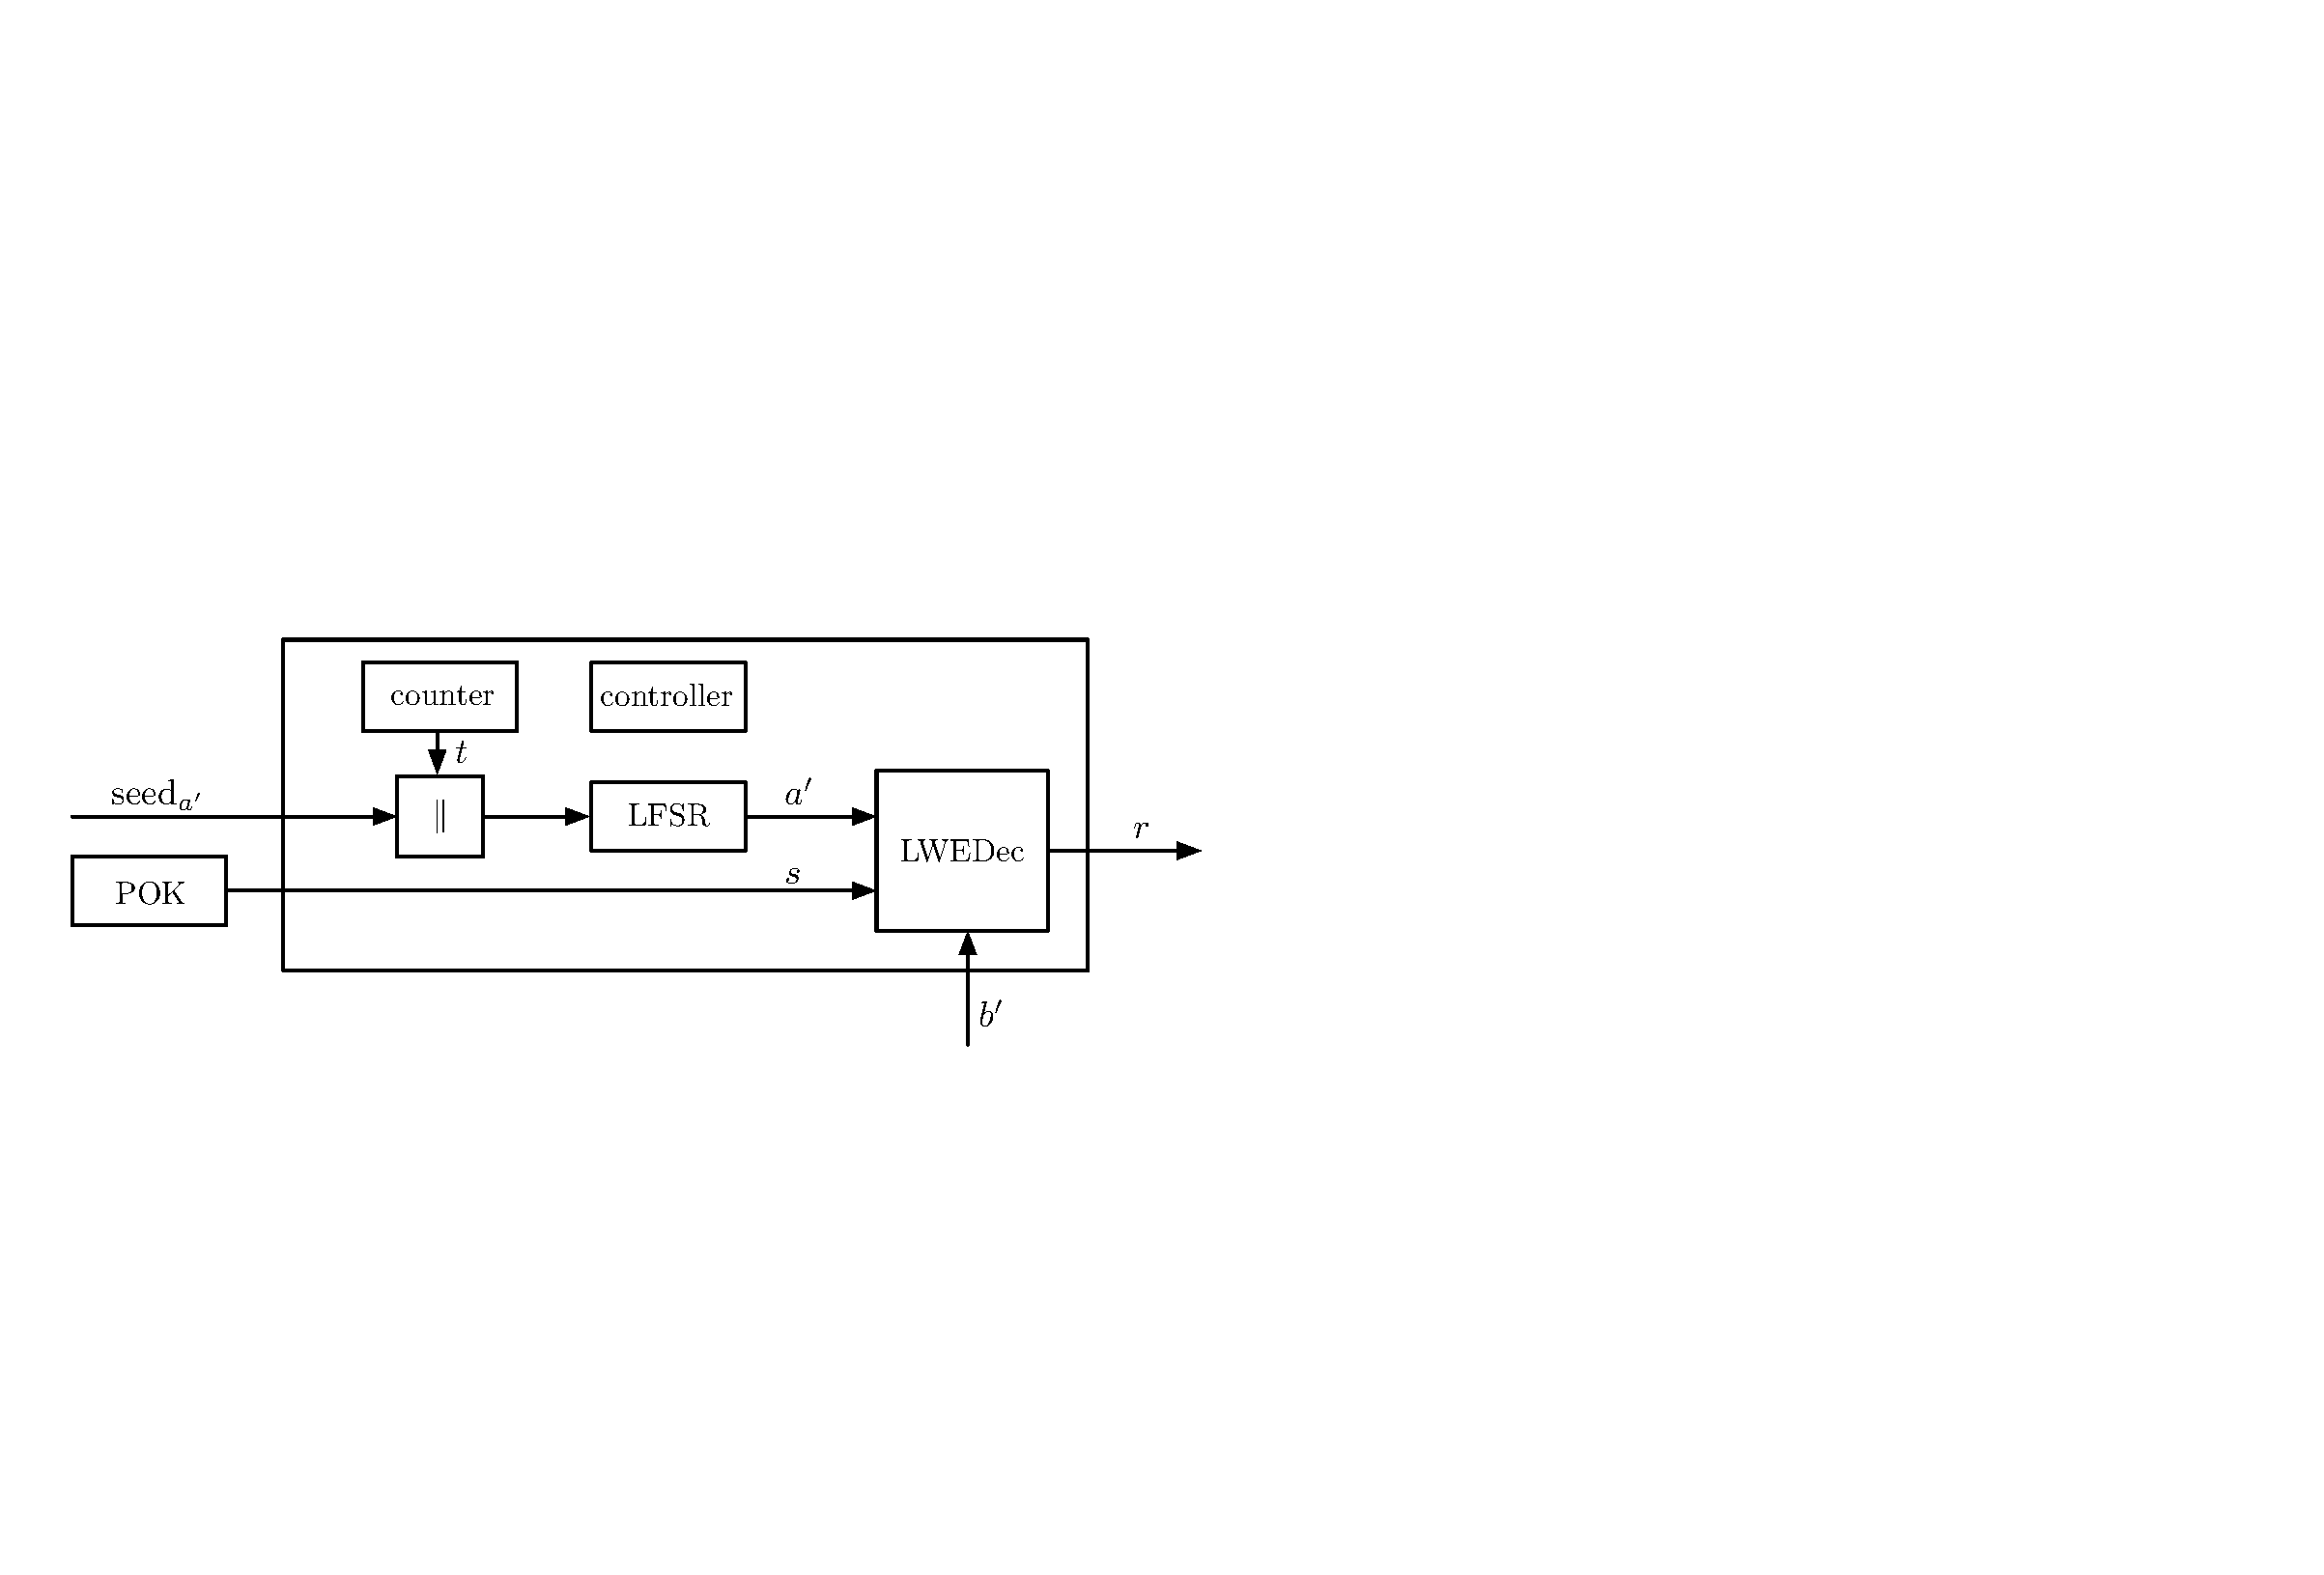
\includegraphics[width = 1.0\linewidth]{./figs/top_level_arch_redraw.pdf}    \caption{Top-level architecture and data flow of the lattice PUF.}
    \label{fig:fpga_impl}
\end{figure}
%\textcolor{red}{The theoretical security guarantees in Section \ref{sec:lwe} shows that an LWE decryption function can be used as a strong PUF with challenges generated from a ciphertext distribution. 
%In this section, we first derive design parameters for the LWE decryption function and show that such a direct implementation of lattice PUF is inefficient in resource constrained environments due to high-ratio of ciphertext to plaintext. 
%As we will illustrate in the following, an LWE decryption function with a 128-bit concrete ML hardness requires transmitting $128.8K$ challenge bits in order to produce a $100$-bit response string. We then solve this problem \emph{by exploiting distributional relaxations allowed by recent work in space-efficient LWEs}. The proposed strategy allows introducing a low-cost PRNG based on an LFSR and transmitting only a small seed, which results in a dramatic reduction of effective challenge size. Next, we introduce a simple defense to protect our PUF against a standard active attack on the LWE decryption function. We then demonstrate two parallelization strategies that reduce response latency. Finally, we introduce a RFE, which is a low-overhead fuzzy extractor, and show its use in an end-to-end authentication scheme.}

The top-level architecture of the proposed lattice PUF is shown in Figure \ref{fig:fpga_impl}.



\subsection{Construct Strong PUF from LWE Decryption Function}
\label{sec:lwe_dec}
\begin{figure}[t!]
    \centering
    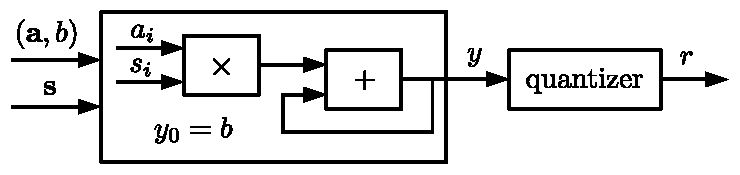
\includegraphics[width = 0.8\linewidth]{./figs/lwe_dec.pdf}
    \caption{Architecture of LWE decryption function.}
    \label{fig:lwedec}
\end{figure}

Figure \ref{fig:lwedec} shows the architecture of LWE decryption function. 
It takes a binary challenge vector $\mathbf{c} = \{c_0,c_1,\ldots,c_{N-1}\}$ of size $N = (n+1)\log q$ which maps to a ciphertext $(\mathbf{a},b)$ in the following way:
\begin{align*}
a_i &= \sum_{j=0}^{\log q-1}c_{(i-1)\log q+j}2^j,\; \forall i\in \{1,2,\ldots,n\}, \\
b &= \sum_{j=0}^{\log q-1}c_{n\log q+j}2^j. 
\end{align*}
Here $a_i$ denotes the $i$-th element of the integer vector $\mathbf{a}\in\mathbb{Z}_q^n$.
In this paper, without specification, $\log(x)$ refers to $\log_2(x)$.
Similarly, the private key $\mathbf{s}$ for the corresponding LWE decryption function is realized by a binary secret key $\mathbf{W} =\{W_0,W_1,\ldots,W_{n\log q-1}\} $ of size $n\log q$:
\begin{equation*}
s_i=\sum_{j=0}^{\log q-1} W_{(i-1)\log q+j} 2^j,\; \forall i\in \{1,2,\ldots,n\}.
\end{equation*}
A modulo-dot-product $b-\innerprod{\mathbf{a},\mathbf{s}}$ is computed using the modulo-multiply-accumulate unit. 
It can be implemented in a serial way using $n$ stages. 
Recall that all additions and multiplications are performed in modulo $q$.
Since $q$ is a power of $2$ in our construction, modulo addition and multiplication can be naturally implemented by integer addition and multiplication that keep only the last $\log q$-bit result. 
Finally the response $r$ is produced by a quantization operation $r = Q(b-\innerprod{\mathbf{a},\mathbf{s}})$: 
\begin{equation*}
Q(x) = \begin{cases}
	0& x \in [0,\frac{q}{4}]\cup(\frac{3q}{4},q-1],\\
	1& x \in (\frac{q}{4},\frac{3q}{4}].
\end{cases}
\end{equation*}

The computation above can be directly implemented as a strong PUF with $2^N$ CRPs since it maps a challenge vector $\mathbf{c}\in \{0,1\}^N$ into a binary response $r\in\{0,1\}$.
We now discuss parameter selection for the LWE decryption function. 
In general, we seek to find design parameters such that 
(1) the resulting PUF has excellent statistical properties, such as uniformity, uniqueness, and reliability, 
(2) successful ML attacks against it require an un-affordably high time complexity in practice, and 
(3) its hardware implementation costs are minimized. 

Prior theoretical arguments establish the impossibility of a polynomial-time attacker. 
To guarantee practical security, we need to estimate the number of samples and the actual running time (or a number of CPU operations) required for a successful ML attack. \cite{regev2009lattices} shows that a small number of samples are enough to solve an LWE problem, but in an exponential time. 
Thus, we refer to runtime as concrete ML resistance (or ML hardness) and say that a PUF has $k$-bit ML resistance if any successful ML attack requires at least $2^k$ operations. 
We adopt the estimator developed by Albrecht \emph{et al.} \cite{albrecht2015concrete} to estimate concrete ML hardness. 
The concrete hardness of an LWE problem increases with the increase of LWE parameters $n$, $q$, and $\alpha$ for all types of attacks.
Recall that $n$ represents the lattice dimension, $q$ represents the range of integer for each dimension, and $\alpha$ reflects the noise level in CRP (ciphertext) generation.
For a given set of parameters, the estimator compares the complexity of several most effective attacks, including decoding, basis reduction, and meet-in-the-middle attacks %\cite{chen2011bkz,howgrave2007hybrid,lindner2011better}. 
\cite{howgrave2007hybrid,lindner2011better}. 
We utilize the estimator in a black-box fashion to find the set of parameters with the target of $128$-bit concrete ML resistance. 

We consider two metrics of implementation cost, both of which scale with $n$: the number of challenge and secret bits needed ($n\log q$), and the number of multiply-accumulate (MAC) operations ($n$).
This motivates the need to decrease $n$.
%\begin{figure}[t!]
%\centering
%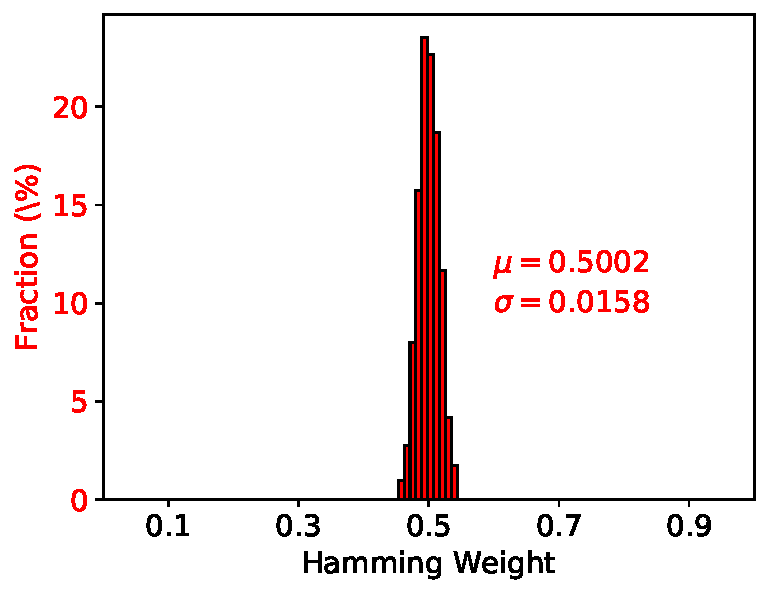
\includegraphics[width = 0.55\linewidth]{./figs/1_bit_HW}
%\caption{CRPs changes radically even with 1 bit POK change.}
%\label{fig:1_bit_hw}
%\end{figure}

%For conventional PUFs, such as APUF and SRAM PUF, an output error is due to environmental noise, e.g. delay changes in APUF and FET strength changes in SRAM PUF with both voltage and temperature.
%In contrast, 
Output errors of the lattice PUF come from two sources: (1) environmental errors of secret bits, and (2) errors of decryption during response generation.
The former can be thought as the failure of key reconstruction in POKs.
Figure \ref{fig:1_bit_hw} shows the hamming-distance between CRPs generated using error-free POKs and POKs with 1 bit error.
Since a single bit-flip completely changes the challenge-response behavior of LWE decryption function, the failure rate of key reconstruction needs to be low, e.g. $10^{-6}$ (as widely adopted in other PUF applications \cite{maes2012pufky}).
Section \ref{sec:result} describes how the target failure rate can be achieved via a conventional FE based on the error-correcting codes.
The latter corresponds to the decryption error and is orthogonal to errors in the secret key $\mathbf{s}$. 
Recall that in CRP generation of the lattice PUF, a bit of plaintext $r$ is sampled and the ciphertext $\mathbf{c}$ is produced by a noisy encryption function $\mathbf{c}=\Enc(r)$. 
Given ciphertext $\mathbf{c}$ as input challenge, the decryption function can output a wrong response $r^\prime\neq r$ when the accumulated error $\sum_{i\in S} e_i$ in the encryption function exceeds the decision boundary.

%\begin{figure}[t!]
%\centering
%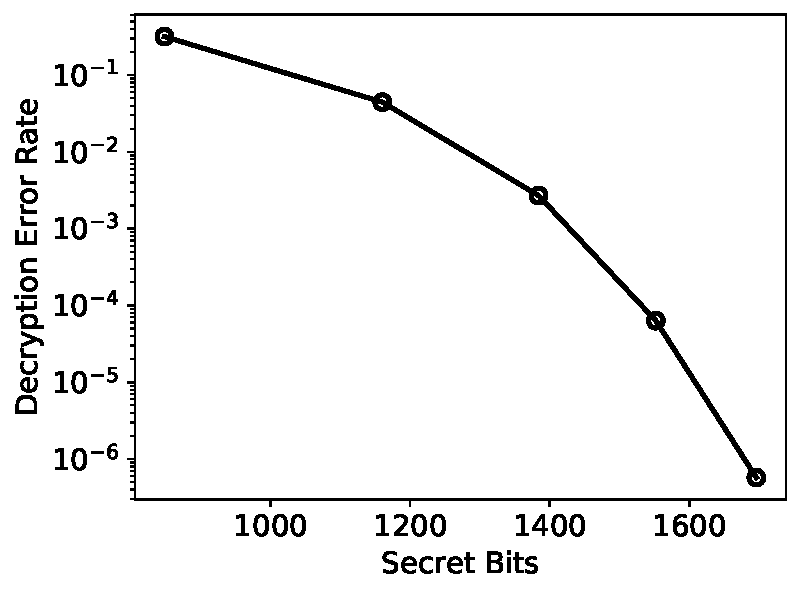
\includegraphics[width = 0.55\linewidth]{./figs/dec_error_secret_bits}
%\caption{Super-exponential decrease of decryption error rate with the increase of secret bits.
%The analysis is done for 128-bit concrete hardness.}
%\vspace{-1.0em}
%\label{fig:num_POK_vs_dec_err}
%\end{figure}

\begin{figure}[t!] 
    \centering
  \subfloat[\label{fig:1_bit_hw}]{%
       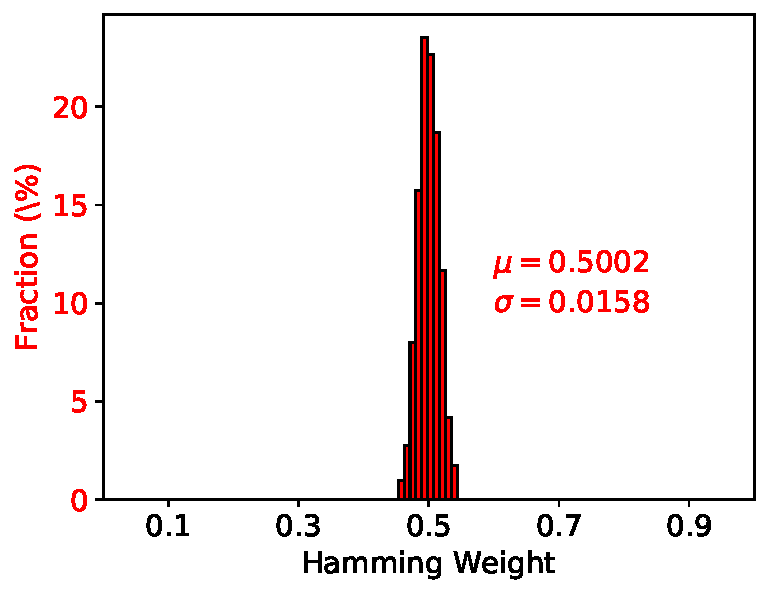
\includegraphics[width=0.48\linewidth]{./figs/1_bit_HW}}
    \hfill
  \subfloat[\label{fig:num_POK_vs_dec_err}]{%
        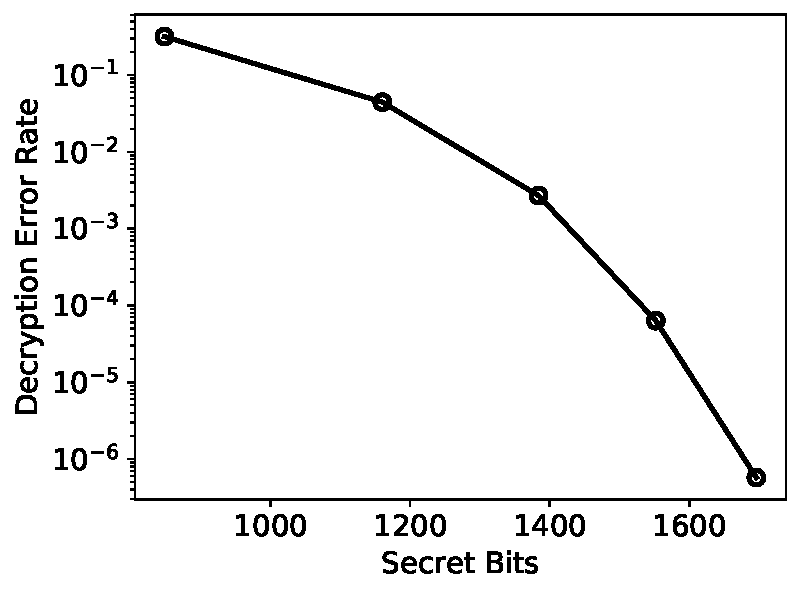
\includegraphics[width=0.5\linewidth]{./figs/dec_error_secret_bits}}
  \caption{(a) CRPs change radically even with 1 bit POK change. (b) Super-exponential decrease of decryption error rate with the increase of secret bits. The analysis is done for 128-bit concrete hardness.}
  \label{fig: lattice_puf_features} 
\end{figure}

%The model for evaluating the decryption error rate is shown in Section \ref{sec:bg}.
In order for a strong PUF to be used in direct authentication, its decryption error rate should be small enough for reliable distinguishability of long strings.
We set the target around $2\%$.
Figure \ref{fig:num_POK_vs_dec_err} explores the trade-off between the number of secret bits and the decryption error rate needed for $128$-bit concrete ML hardness.
It shows that, at fixed concrete ML hardness, the decryption error rate decreases super exponentially with the number of secret bits. 

Considering the design metrics above, a feasible set of parameters is found using the estimator in \cite{albrecht2015concrete}.
By setting $n=160$, $q=256$, $m=256$ and $\alpha = 2.20\%$, we achieve a lattice PUF with $128$-bit concrete hardness and a decryption error rate of $1.26\%$.

In order to get a $1$-bit response, $(n+1)\log q = 1288$ bits need to be sent to the lattice PUF as a challenge.
For direct authentication applications, usually around $100$ bits of responses are required. Therefore, the direct implementation described so far would require $C = 128.8K$ challenge bits.
This high ratio of challenge length to response length limits its practical use in many scenarios when communication is expensive.

%\textcolor{red}{A class of attacks which manipulates public helper data to exploit PUF generated keys can compromise PUF security \cite{helper_data_manipulation}. Such attacks apply to pairing-based PUFs (for instance, RO PUFs), and require public access to helper data. However, such attacks may not be applicable to our construction, since our POK is based on the SRAM PUF, which follows a completely different mechanism. In addition, the possibility of the attacks can be reduced by limiting public access to helper data. Therefore, the helper data manipulation attack is not a major concern for our design.}


\vspace{-0.5em}
\subsection{Challenge Compression through Distributional Relaxation}
\label{sec:lfsr}
%We now describe the proposed strategy based on space-efficient LWE that overcomes the limitation on communication inefficiency.
The LWE decryption function described in Section \ref{sec:lwe_dec} requires a challenge $\mathbf{c}$ in the form $\mathbf{c}=(\mathbf{a},b)$ to be sent from the server to the PUF. 
To represent vector $\mathbf{a} \in \mathbb{Z}_q^n$ requires $n\log q$ bits while to represent scalar $b \in \mathbb{Z}_q$  requires only $\log q$ bits. 
Thus, the major cost of transmission lies in sending $\mathbf{a}$. 
We wish to avoid sending $\mathbf{a}$ directly and, instead, to send a compressed (shorter) version of $\mathbf{a}$  and re-generate its full-size version on the PUF.
Our approach is enabled by the recent results on the distributional behavior of $\mathbf{a}=\mathbf{A}^T\mathbf{x}$ \cite{akavia2009simultaneous} and the concept of space-efficient LWE \cite{galbraith2013space}.

Recall that $b$ is given by: 
\begin{align*}
    b&=\mathbf{b}^T\mathbf{x}+r\floor{q/2}\\
    &= (\mathbf{A}\mathbf{s}+\mathbf{e})^T\mathbf{x}+r\floor{q/2}\\
    &=(\mathbf{A}^T\mathbf{x})^T\mathbf{s}+\mathbf{e}^T\mathbf{x}+r\floor{q/2}.
\end{align*}
First, we replace the component $\mathbf{a}=\mathbf{A}^T\mathbf{x}$ by $\mathbf{a}^*$ uniformly randomly sampled from $\mathbf{Z}_q^n$. That allows us to represent challenge $\mathbf{c} = (\mathbf{a},b)$:
\begin{equation*}
    \begin{cases}
    \mathbf{a}= \mathbf{A}^T\mathbf{x}\\
    b = (\mathbf{A}^T\mathbf{x})^T\mathbf{s}+\mathbf{e}^T\mathbf{x}+r\floor{q/2}
    \end{cases}
\end{equation*}
as $\mathbf{c}^*=(\mathbf{a}^*,b^*)$:
\begin{equation*}
    \begin{cases}
    \mathbf{a}^*\\
    b^*=\mathbf{a}^{*T}\mathbf{s}+\mathbf{e}^T\mathbf{x}+r\floor{q/2}
    \end{cases}.
\end{equation*}
In \cite{akavia2009simultaneous}, it is proven that distribution of $\mathbf{c}^*=(\mathbf{a}^*,b^*)$ is statistically close to the original ciphertext distribution, therefore the required security properties are preserved.  

The advantage of the above approximation is that, as shown by \cite{galbraith2013space}, several low-complexity  PRNGs are capable of producing an output string $\mathbf{a}^\prime$ suitably close to $\mathbf{a^*}\in\mathbb{Z}^n_q$ within the context of LWE cryptosystem. In particular, an LFSR is an especially simple PRNG having the right properties.
Specifically, a vector $\mathbf{a}^\prime$ generated by an LFSR provides similar concrete security guarantees against standard attacks on LWE, such as CVP reduction, decoding, and basis reduction \cite{galbraith2013space}.
This is because LFSR-generated $\mathbf{a}^\prime$ maintains good properties including:
\begin{itemize}
    \item it is hard to find ``nice'' bases for a lattice with basis from LFSR-generated $\mathbf{a}^\prime$;
    \item given an arbitrary vector in $\mathbb{Z}_q^n$, it is hard to represent it as a binary linear combination of LFSR-generated $\mathbf{a}^\prime$'s;
    \item it is hard to find a short vector $\mathbf{w}$ that is orthogonal to LFSR-generated $\mathbf{a}^\prime$'s.
\end{itemize}

The ability to rely on a simple PRNG to produce $\mathbf{a}^\prime$ allows a dramatic reduction in challenge transfer cost. 
Now, the challenge $\mathbf{c}^\prime$ contains only a small $\text{seed}_{\mathbf{a}^\prime}$ into the PRNG and the corresponding $b^\prime$ as
\begin{align*}
    b^\prime&=(\mathbf{a}^\prime)^T\mathbf{s}+\mathbf{e}^T\mathbf{x}+r\floor{q/2}\\
    &= \LFSR{(\text{seed}_{\mathbf{a}^\prime})}^T\mathbf{s}+\mathbf{e}^T\mathbf{x}+r\floor{q/2}.
\end{align*}
Here $\LFSR(\cdot)$ denotes the output generated by an LFSR.


%\begin{figure*}[t!]
%\centering
%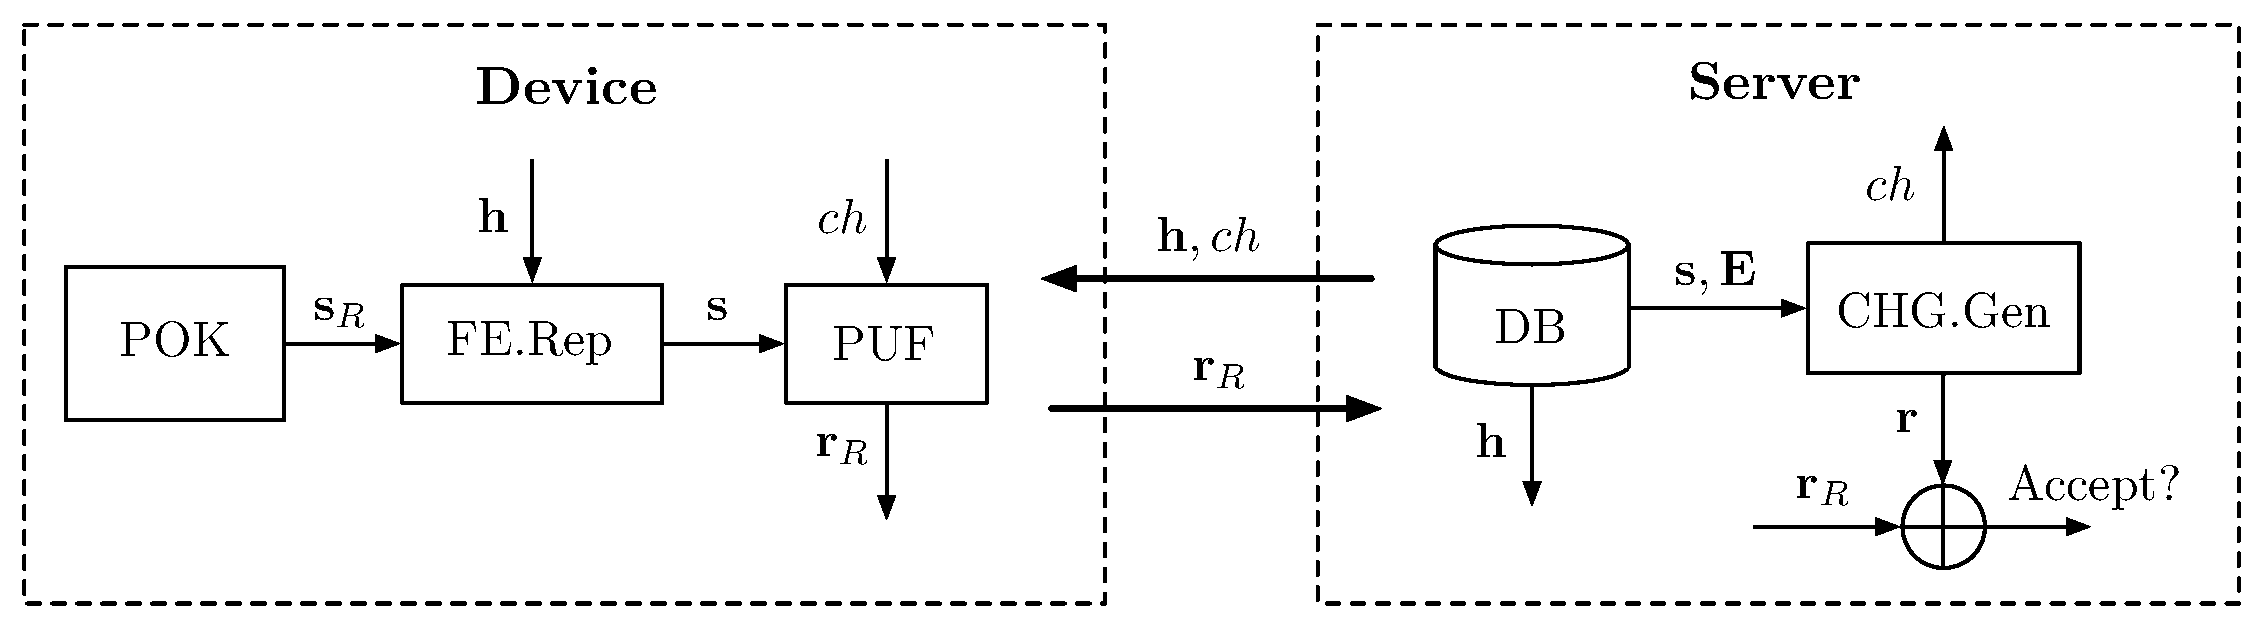
\includegraphics[width = 0.85\linewidth]{./figs/authen_system}
%\caption{Building blocks of the authentication scheme with the lattice PUF.}
%\label{fig:authen_system}
%\end{figure*}

%\begin{figure}[t!]
%\centering
%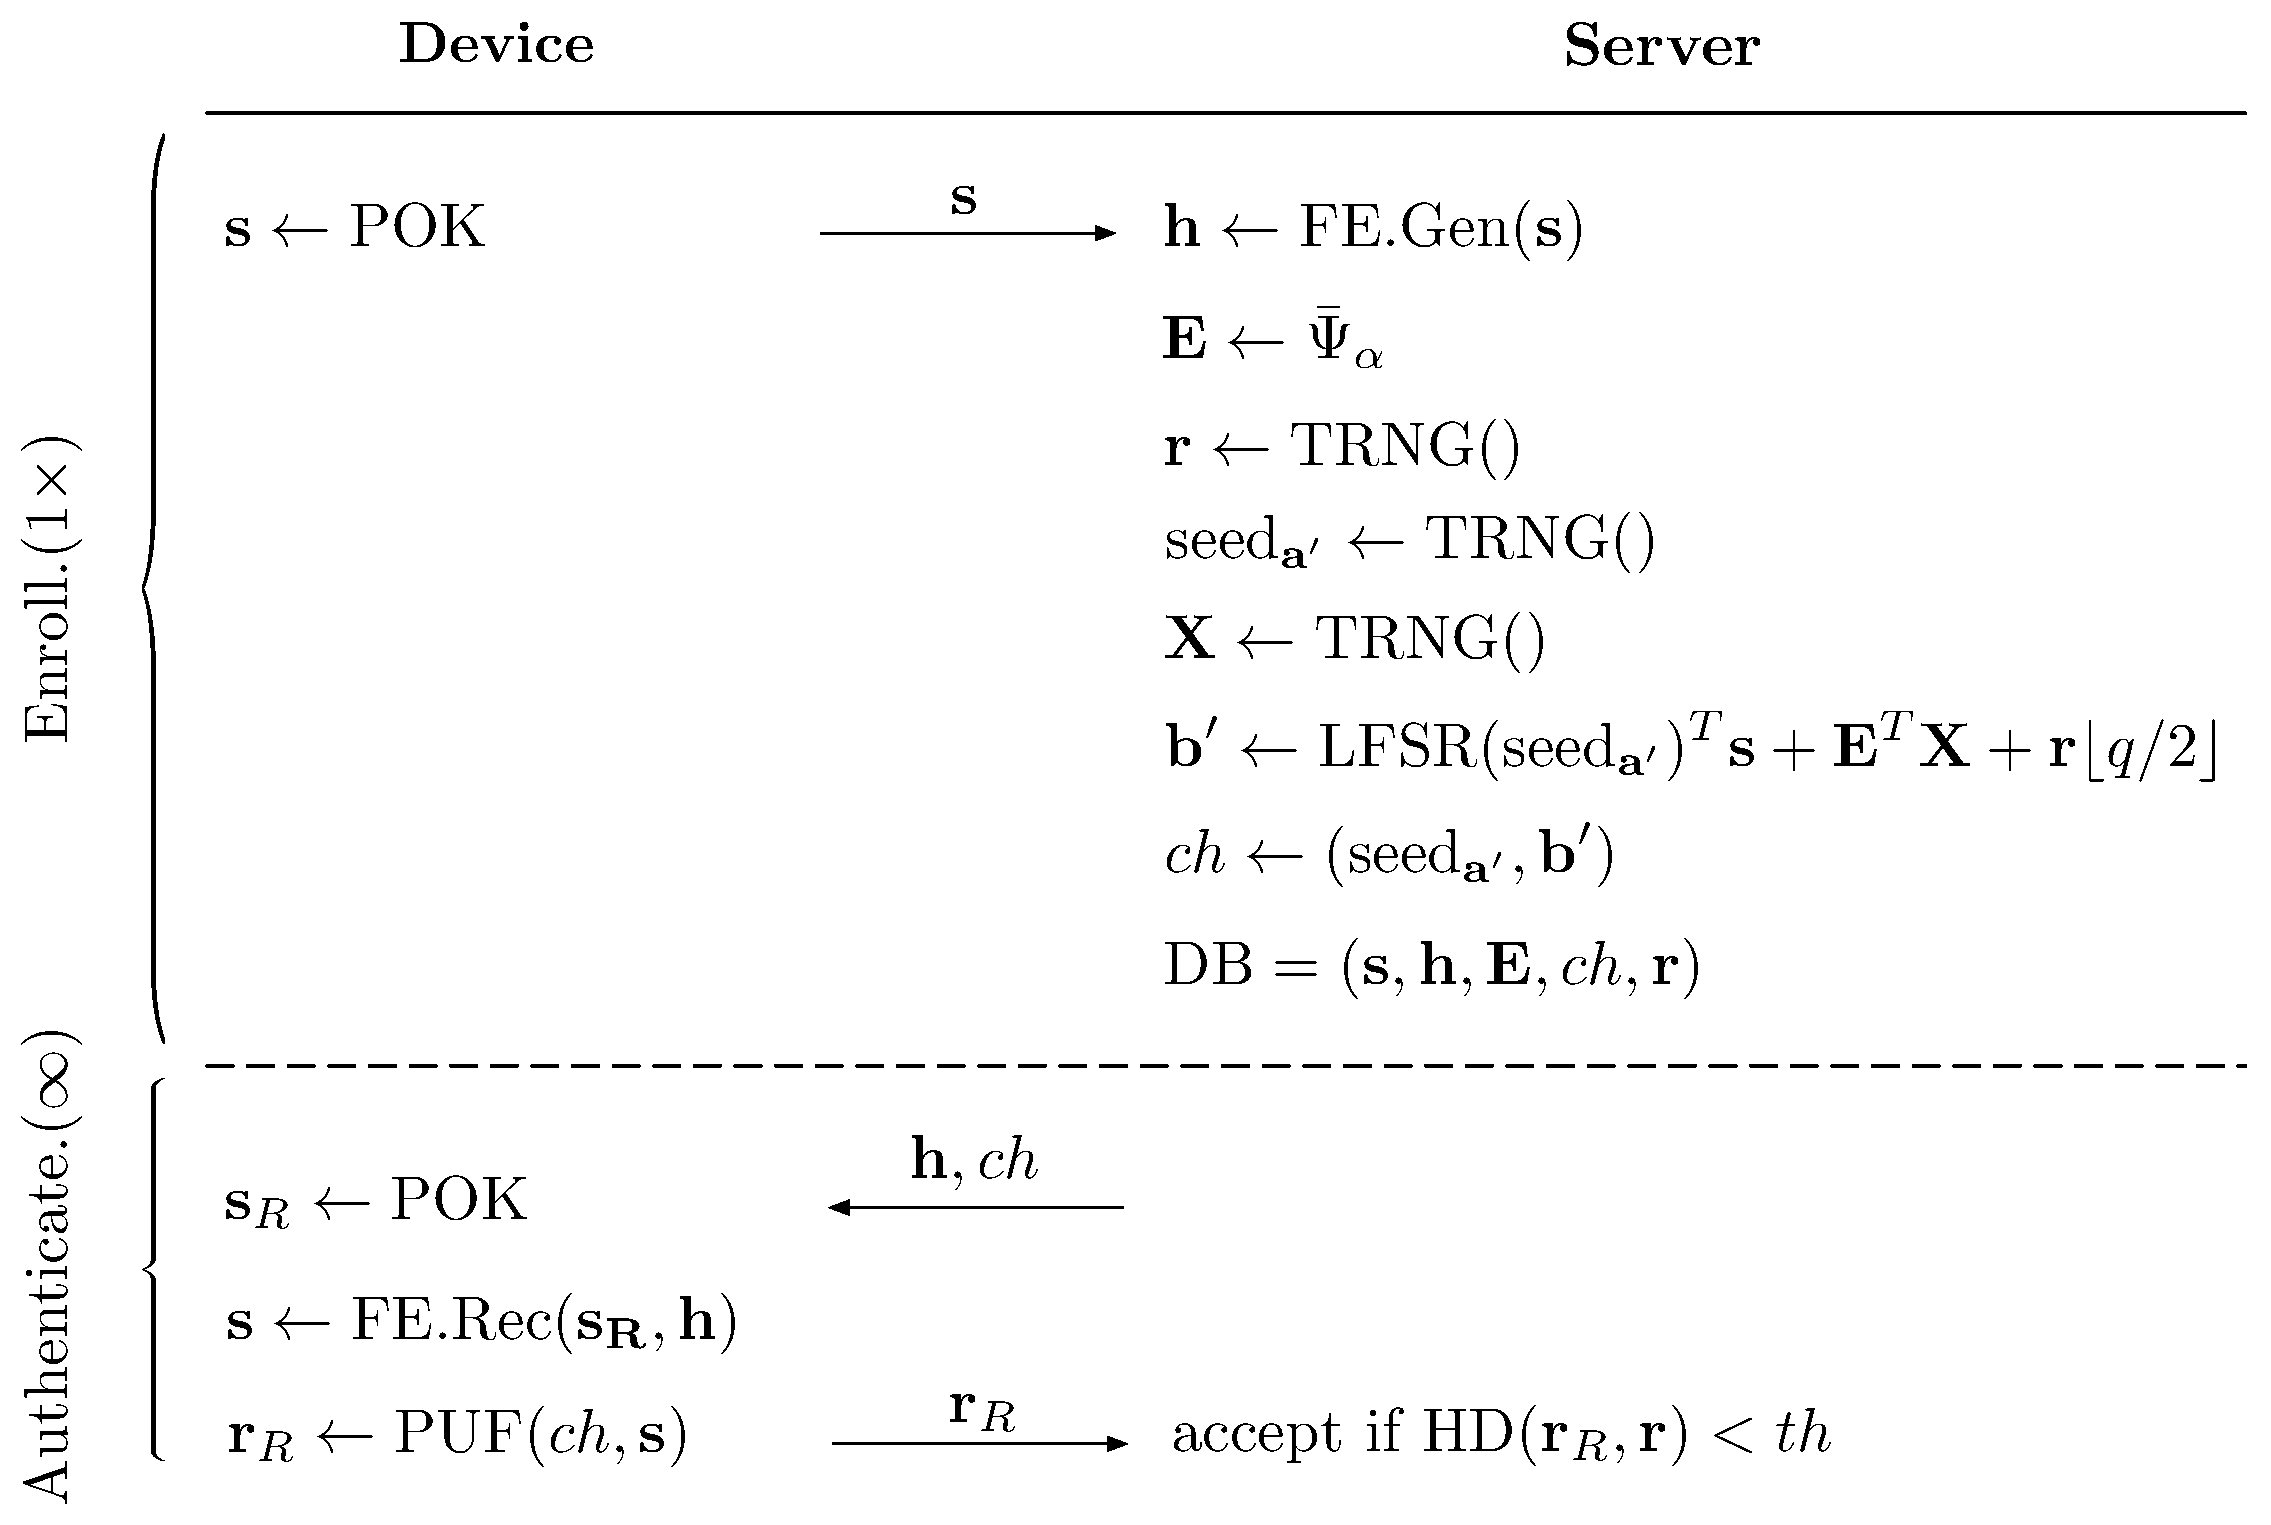
\includegraphics[width = 1.0\linewidth]{./figs/protocol}
%\caption{End-to-end authentication system with the lattice PUF.}
%\label{fig:protocol}
%\end{figure}

With LWE parameters chosen as Section \ref{sec:lwe_dec}, using a seed of length $l=256$ is able to reduce the challenge length from $1288$ to $256+8=264$ per one bit of response. 
The improvement of efficiency becomes more pronounced for generating multiple responses:
This is because $\mathbf{a}^\prime_1 \ldots \mathbf{a}^\prime_t$ can be generated sequentially from the $l$-bit seed, so that only the seed and $b^\prime_1,\ldots, b^\prime_t \in Z_q$ are required to be sent to the PUF side. 
$100$ bits of responses now require only transmitting $256+100\times\log 256 = 1056$ bits for challenges.

\subsection{Countermeasure for Active Attack}
\label{sec:counter}
%The focus of the paper is a PUF secure against passive attacks in which the observed challenges can be used to derive an internal model of the PUF. 
%However, the LWE decryption function is vulnerable to an active attack that supplies arbitrary input challenges. 
%(As we show, this risk also carries into an LFSR-based variant). 

We now demonstrate an active attack that compromises security of lattice PUF. The attack is premised on the ability to supply arbitrary challenges (ciphertexts) as inputs to the decryption function. 
The attack proceeds as follows. 
The attacker fixes $\mathbf{a}$ and enumerates all possible $b\in \mathbb{Z}_q$ for challenge $\mathbf{c} = (\mathbf{a},b)$.
As $b$ increases from $0$ to $q-1$, the response $r = Q(b-\innerprod{\mathbf{a},\mathbf{s}})$ changes from  $Q(b-\innerprod{\mathbf{a},\mathbf{s}}) = 0$ to $Q(b+1-\innerprod{\mathbf{a},\mathbf{s}}) = 1$ exactly when $b$ satisfies
\begin{equation*}
b-\innerprod{\mathbf{a},\mathbf{s}} = q/4.
\end{equation*}
We denote this specific value of $b$ as $\hat{b}$. 
The exact value of $\innerprod{\mathbf{a},\mathbf{s}}$ can then be extracted by $\innerprod{\mathbf{a},\mathbf{s}} = \hat{b} - q/4$. 
By repeating this procedure $n$ times, the attacker is able to set up $n$ linear equations (without errors):  
\begin{align*}
\label{eq:secret_eqs}
    \innerprod{\mathbf{a}_0,\mathbf{s}} &= \hat{b}_0 - q/4, \\
    \innerprod{\mathbf{a}_1,\mathbf{s}} &= \hat{b}_1 - q/4, \\
    & \cdots \\
    \innerprod{\mathbf{a}_{n-1},\mathbf{s}} &= \hat{b}_{n-1} - q/4.
\end{align*}
Gaussian elimination can then be used to solve for $\mathbf{s}$, entailing compromising the system. 
%The reason the attack succeeds is that attackers are able to fix $\mathbf{a}$ and use it for multiple values of $b$. 

%We overcome the risk of such an attack by adopting the technique in \cite{yu2016lockdown}: we introduce a self-incrementing counter to embed the counter value into a challenge seed.
To defend against the attack, we introduce a self-incrementing counter to embed the counter value into a challenge seed \cite{yu2016lockdown}.
This makes the attack impossible as the counter restricts the attacker's ability to completely control input challenges to the LWE decryption function.
As a result, the attacker cannot enumerate all values of $b$ while keeping $\mathbf{a}$ unchanged. 
As shown in Figure \ref{fig:fpga_impl}, the concatenation of the challenger-provided seed and the counter value $t$ (i.e. $\text{seed}_{\mathbf{a}'}||t$) is used as the seed for generating $\mathbf{a}$. 
The counter value is public and is incremented by $1$ on each response generation.

\subsection{Latency Optimization via Design Parallelization}
\label{sec: lpuf_par}


%\begin{figure}[t!]
%\centering
%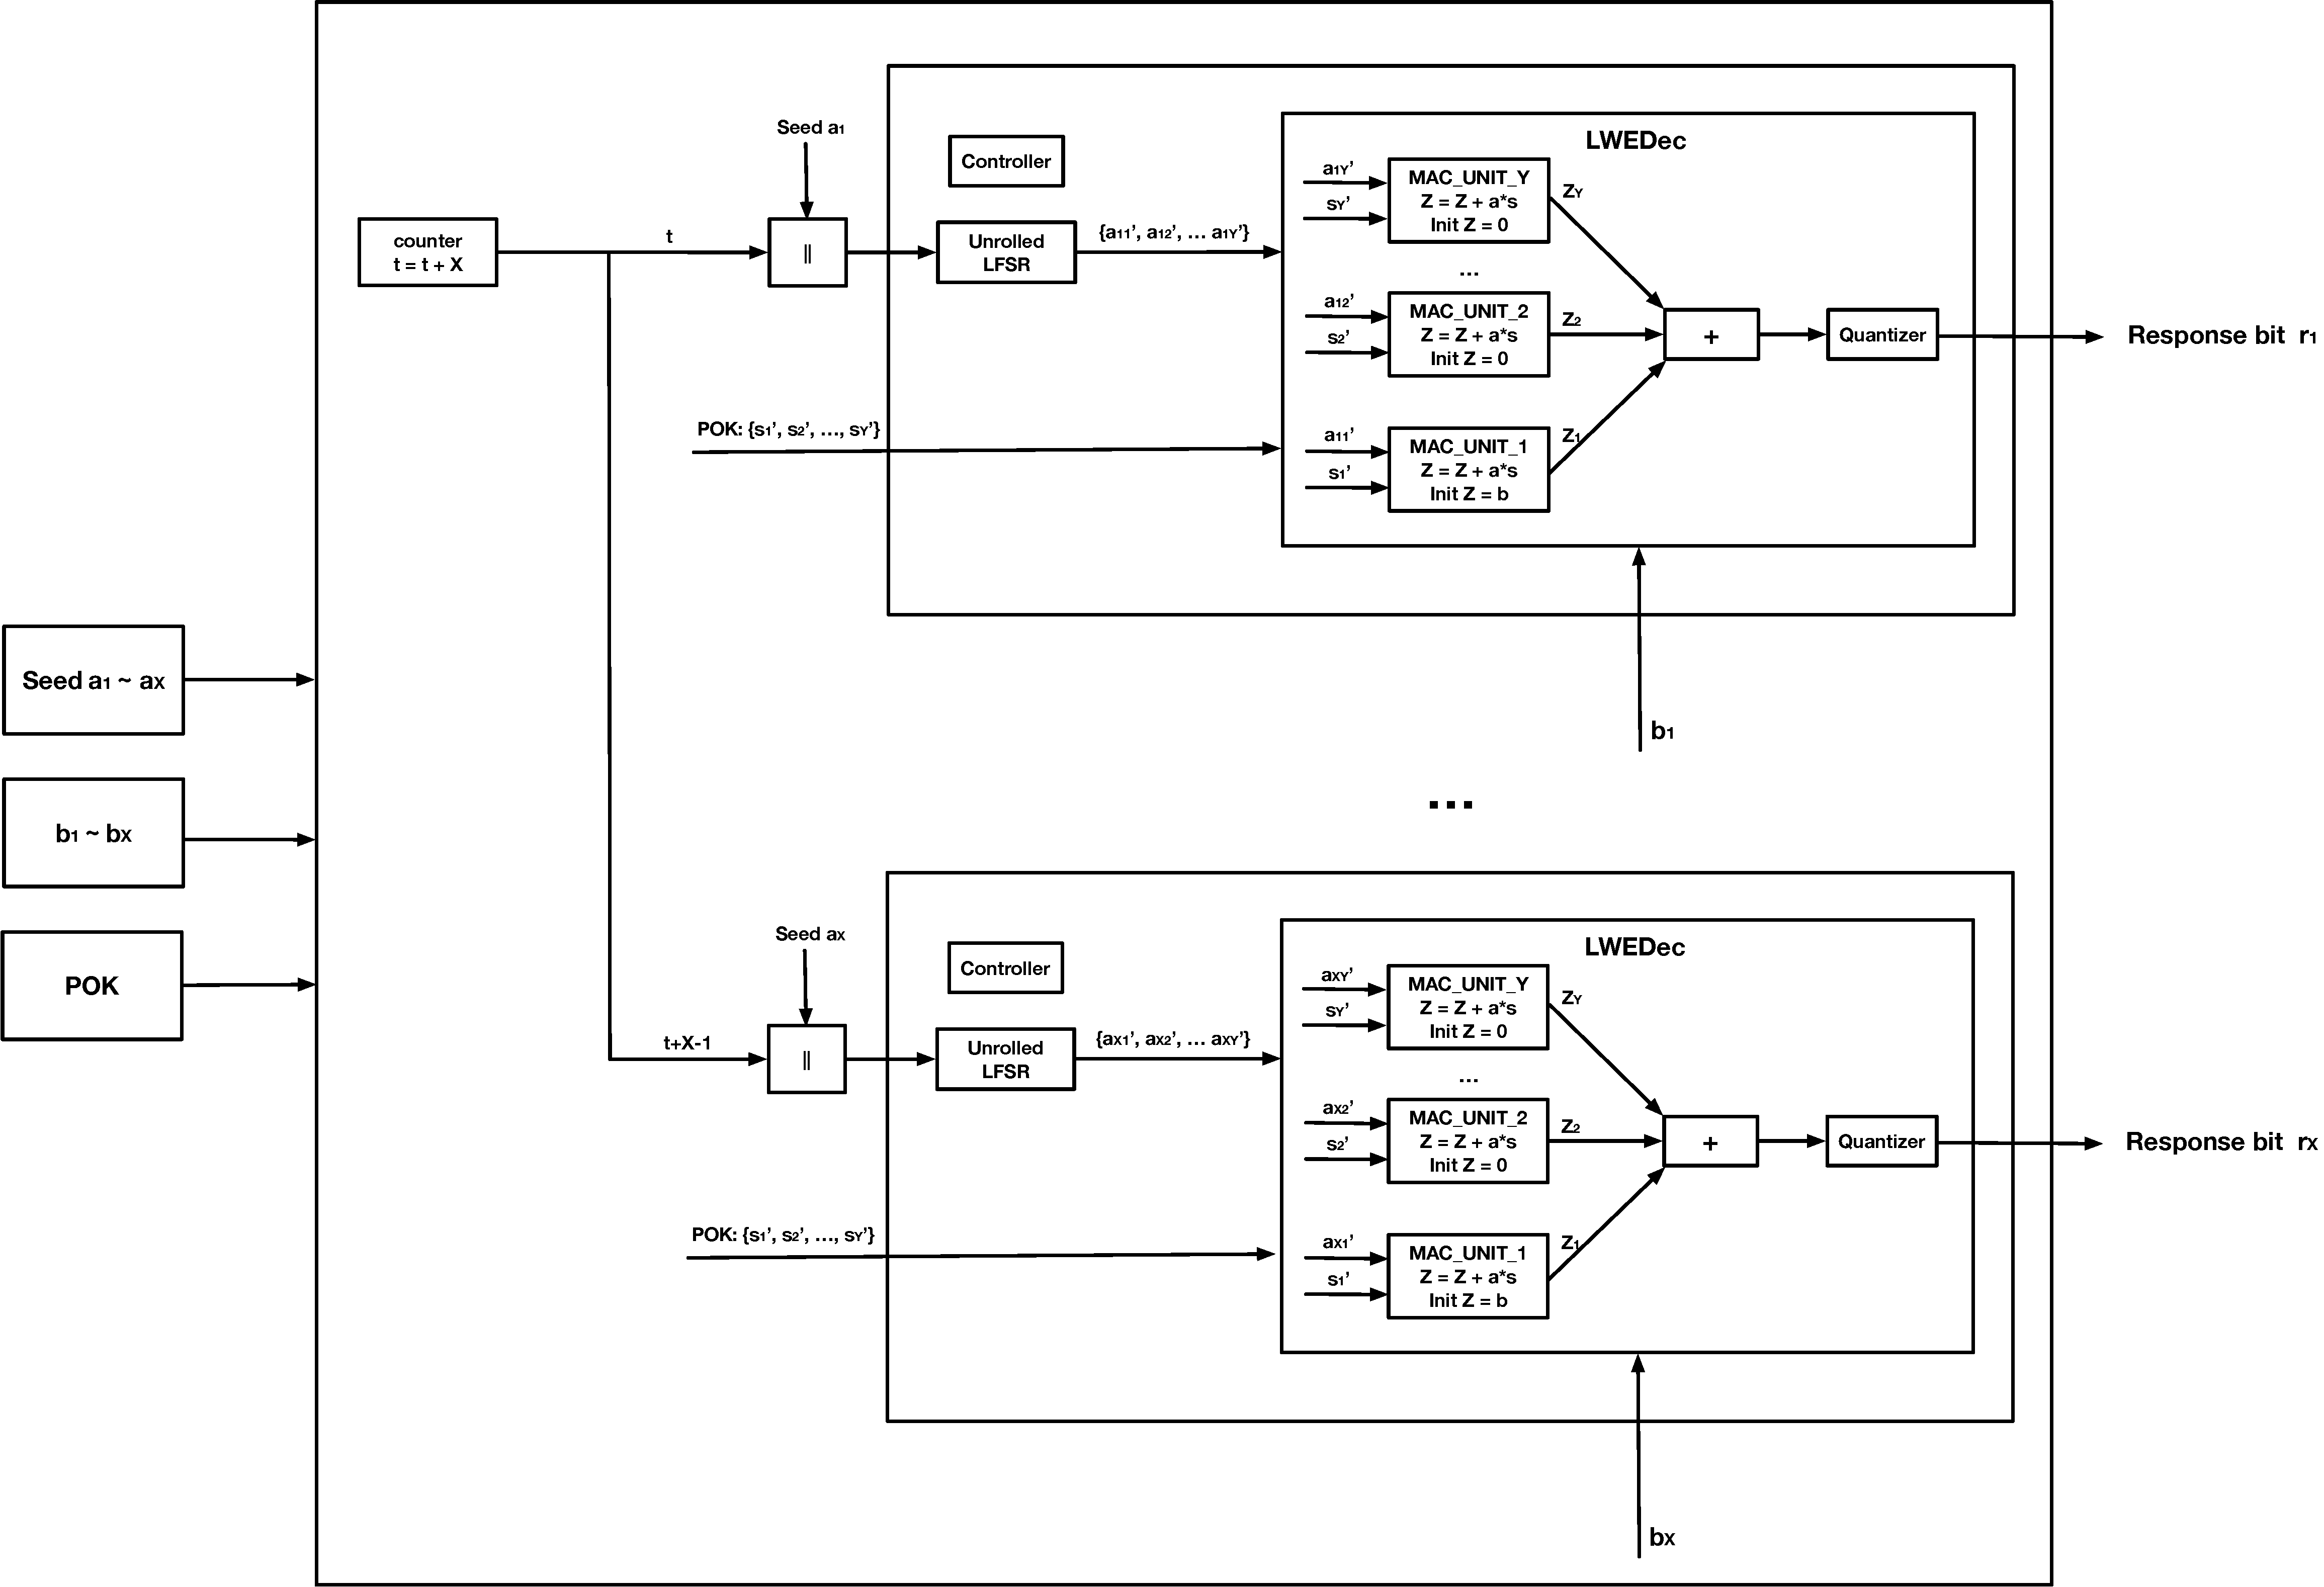
\includegraphics[width = 1.0\linewidth]{./figs/lpuf_p1_p2}
%\caption{Lattice PUF parallelization 3.}
%\label{fig:lpuf_p1_p2}
%\end{figure}

The lattice PUF architecture shown in Fig. \ref{fig:fpga_impl} achieves low hardware implementation cost via a bit-serial design. %The design adopts a single multiply-and-accumulate (MAC) unit and generates a single response bit after multiple sequential MAC operations. 
However, the highly serialized design leads to inefficient utilization of clock cycles resulting in large response latency. To generate one bit of response, the design needs $160$ sequential MAC operations and each MAC needs to wait $8$ cycles until one byte of ciphertext is generated by the bit-serial LFSR. This is undesirable in performance-critical applications. %While the lightweight property is generally desired in a resource constrained environment, latency of response generation is also critical in a PUF-based application. 


We observe that latency is limited by two factors: (1) the LFSR and LWE decryption function (LFSR-LWEDec) datapath produces response bits serially, and (2) the LWE decryption function performs a single MAC sequentially.  We optimize each aspect. %to reduce the overall latency.
%\textcolor{red}{We keep LFSR in the latency-optimized design due to its capability of reducing challenge transmission cost, as illustrated in Section \ref{sec:lfsr}.}

\begin{figure}[t!]
\centering
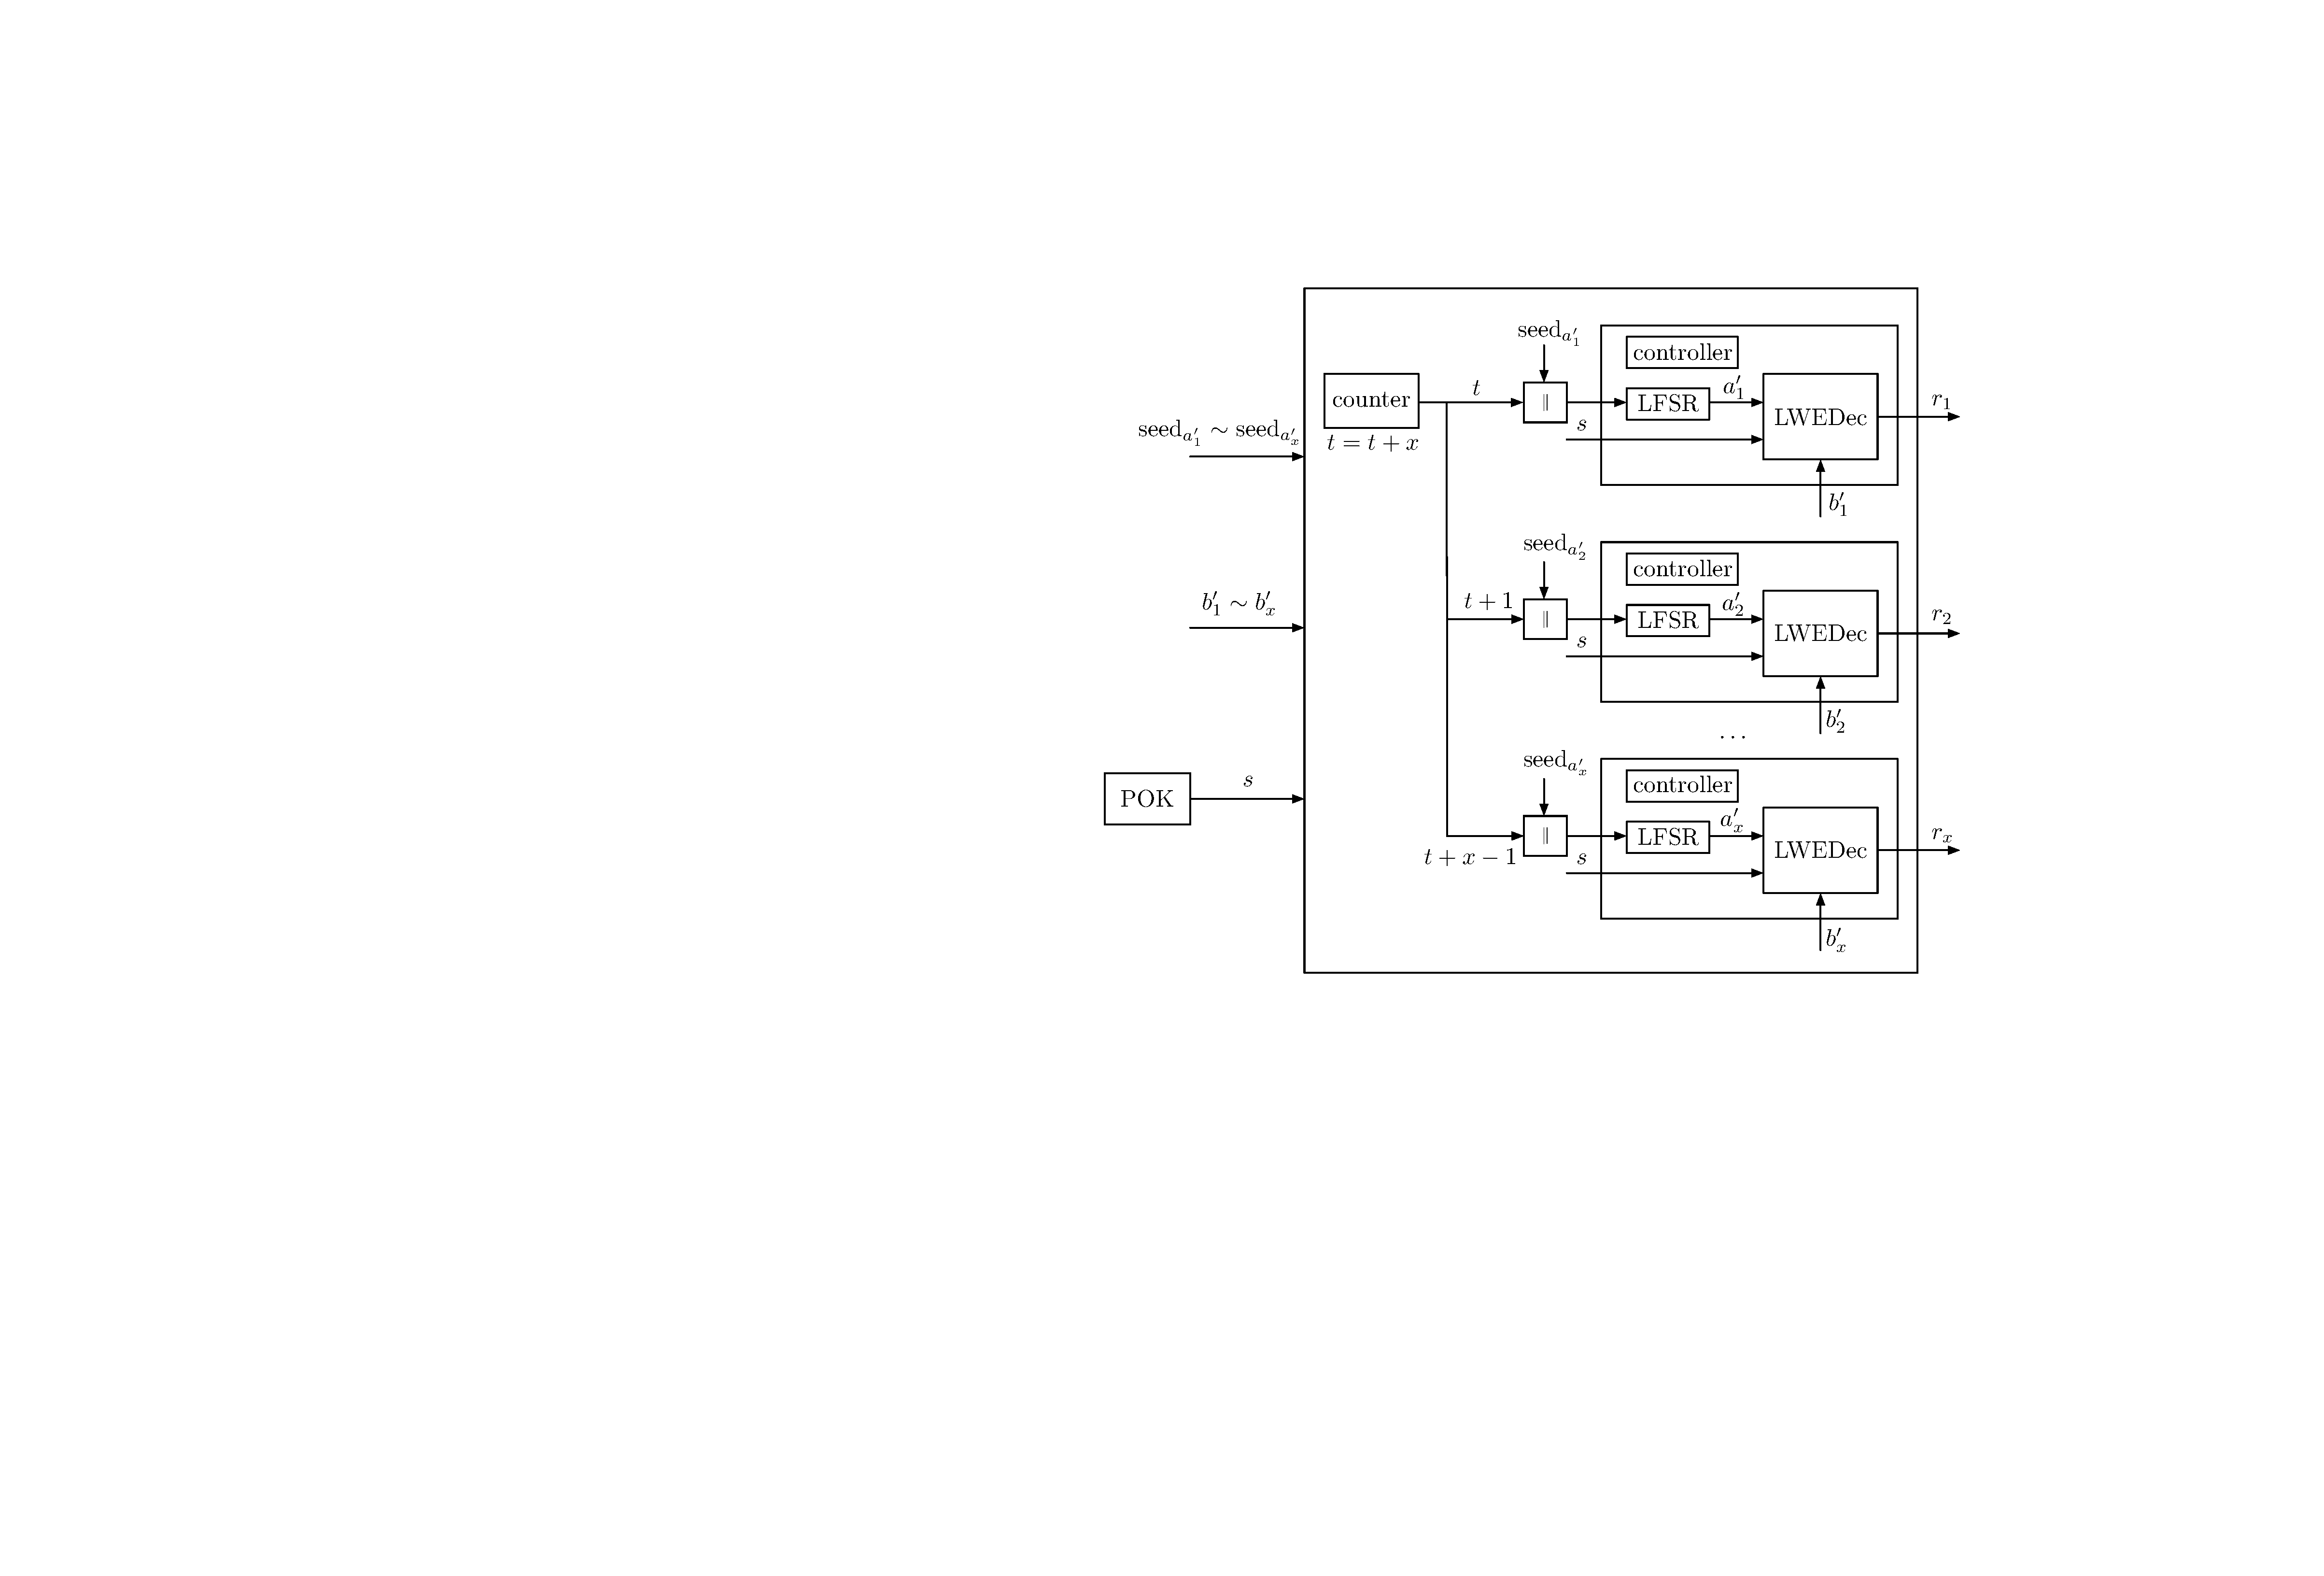
\includegraphics[width = 0.8\linewidth]{./figs/lpuf_p1}
\caption{Reducing latency via a parallel LFSR-LWEDec datapath.}
\label{fig:lpuf_p1}
\end{figure}

We first parallelize the LFSR-LWEDec data-path which implements the functionality in response generation: the LFSR generates ciphertext and LWE decryption function performs modulo MAC operation. Parallelizing it allows multiple response bits to be generated simultaneously, Fig. \ref{fig:lpuf_p1}. Each LFSR-LWEDec data-path uses the same POK, but receives different LFSR seeds and ciphertext inputs. 

We adapt the counter technique described in Section \ref{sec:counter}. %Specifically, we embed an increasing value into the LFSR seed for each LFSR-LWEDec data-path. The increasing values are counted from the output of a main counter, which increments by the number of parallel data-paths for each response generation. 
We embed an increasing counter value into the seed of each datapath, Fig. \ref{fig:lpuf_p1}. %On a design with $P_1$ parallel LFSR-LWEDec data-paths, 
The strategy directly enables $P_1$ times reduction in response generation latency, at the cost of $P_1$ times increase in seed transmission and datapath hardware utilization.

We now investigate how to increase the dot-product throughput in LWE decryption. Since the LWE decryption function contains only a single MAC unit, we increase the number of MACs. However, the throughput of the LFSR limits the overall throughput of the data-path: it produces only a single output bit per cycle. %For each MAC operation, the MAC unit has to wait until a full ciphertext byte ($q=256$) is generated. 
Therefore, to fully utilize the parallel MAC units, the LFSR needs to produce a sufficient number of ciphertext bytes on each cycle. We adopt an unrolled LFSR to increase its throughput.

\begin{figure}[t!]
\centering
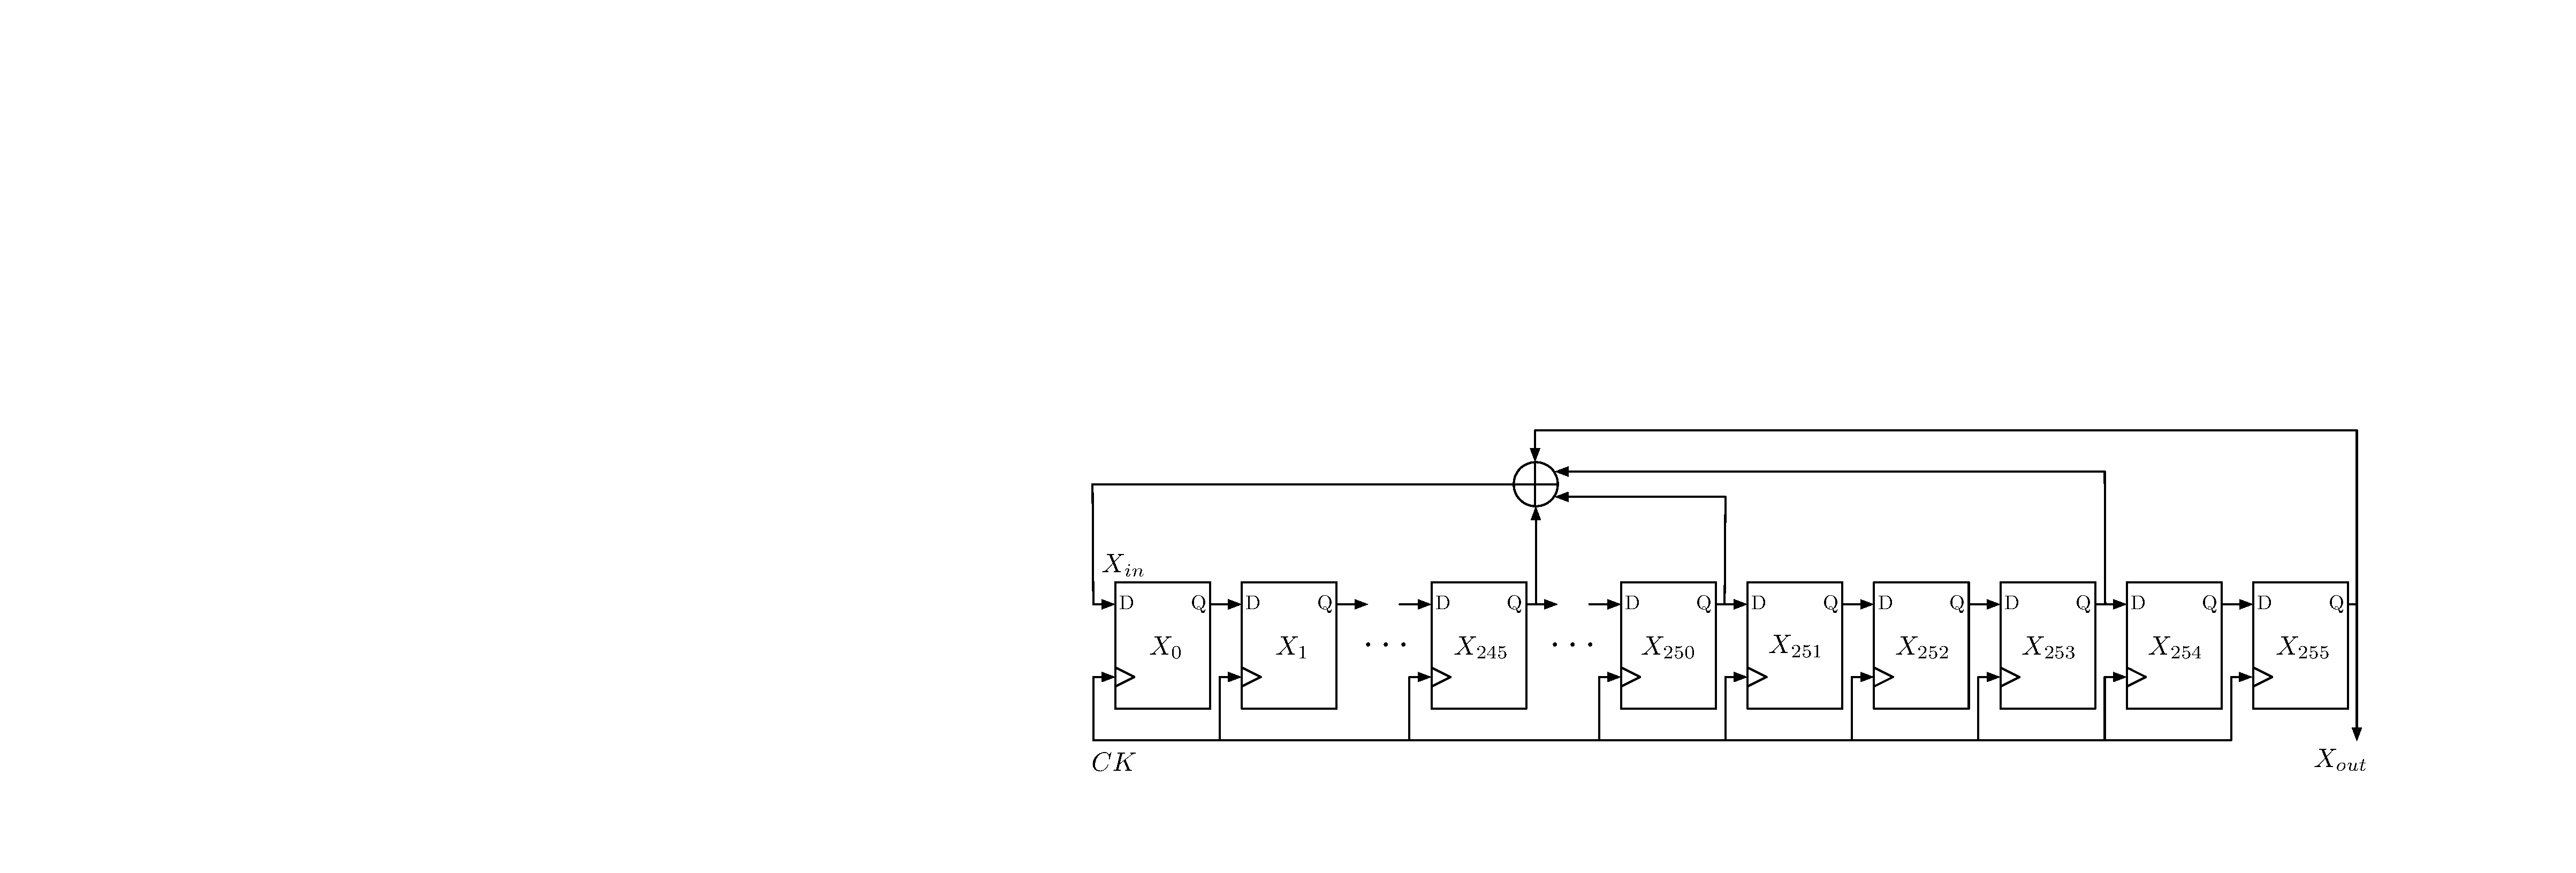
\includegraphics[width = 1.0\linewidth]{./figs/lfsr_baseline_compressed}
\caption{A 256-bit bit-serial LFSR.}
\label{fig:lfsr_baseline}
\end{figure}

\begin{figure}[t!]
\centering
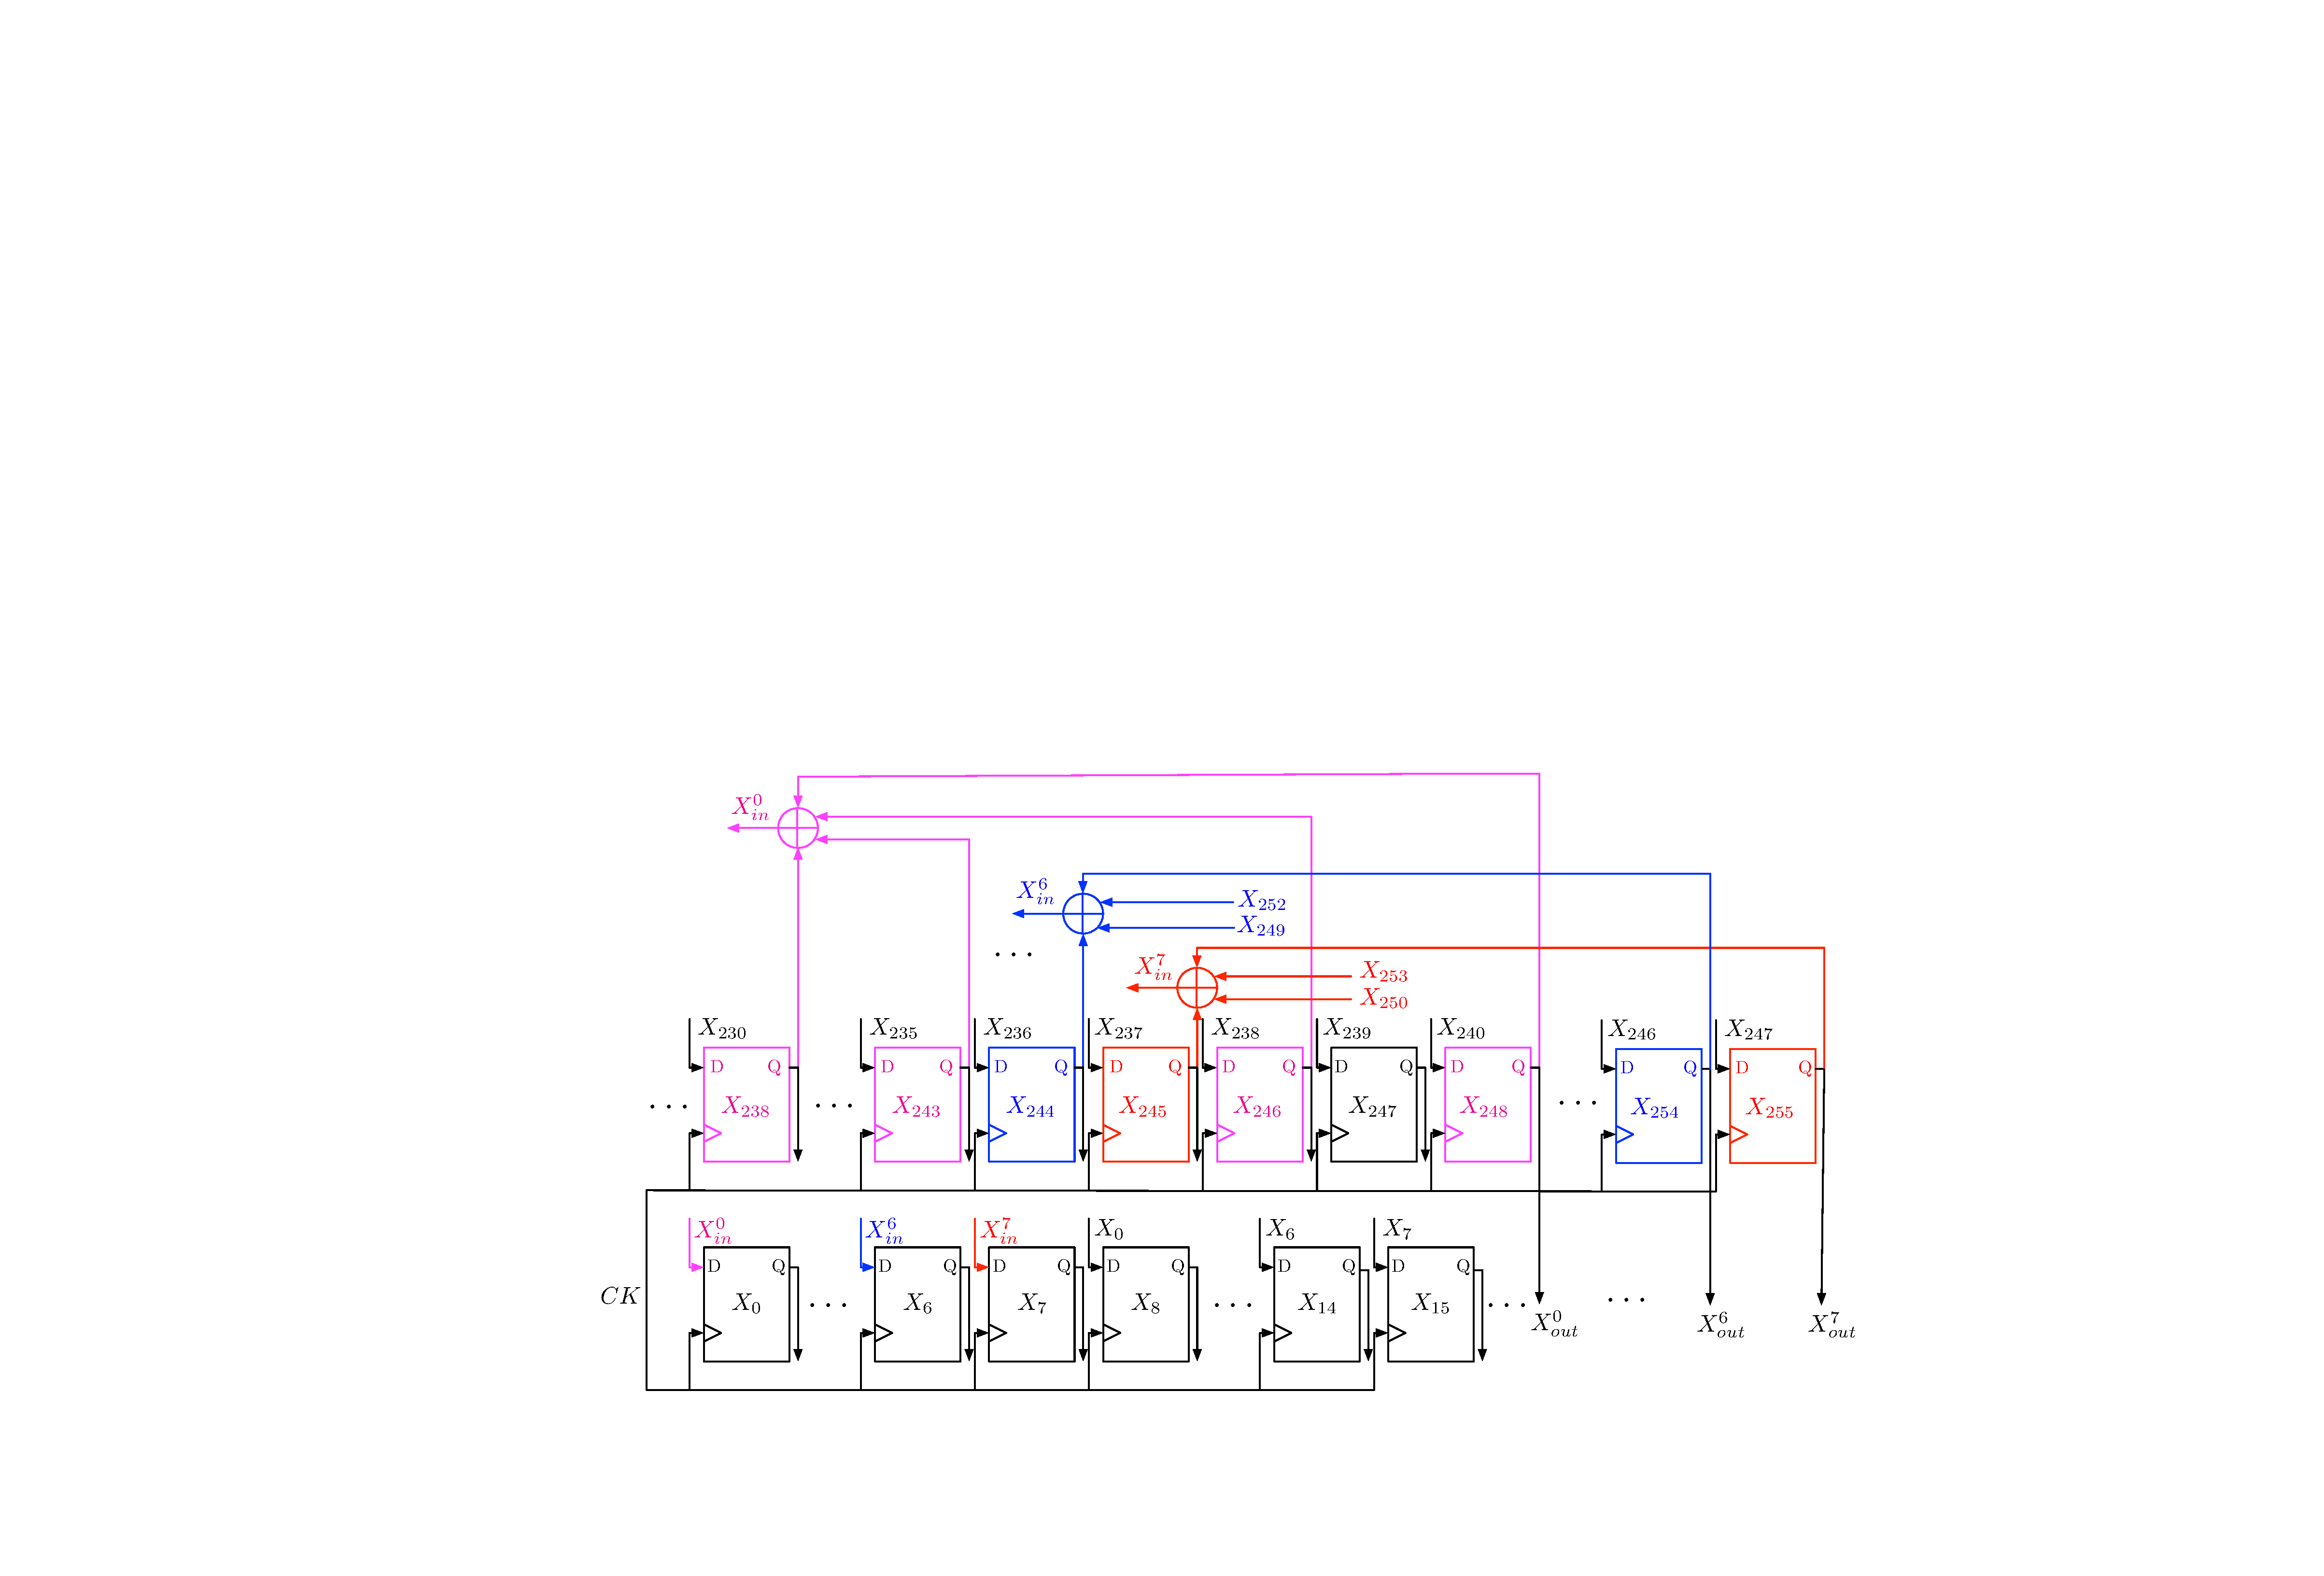
\includegraphics[width = 1.0\linewidth]{./figs/lfsr_unrolled_compressed}
\caption{A 256-bit LFSR unrolled by a factor of 8.}
\label{fig:lfsr_unrolled}
\end{figure}

\begin{figure}[t!]
\centering
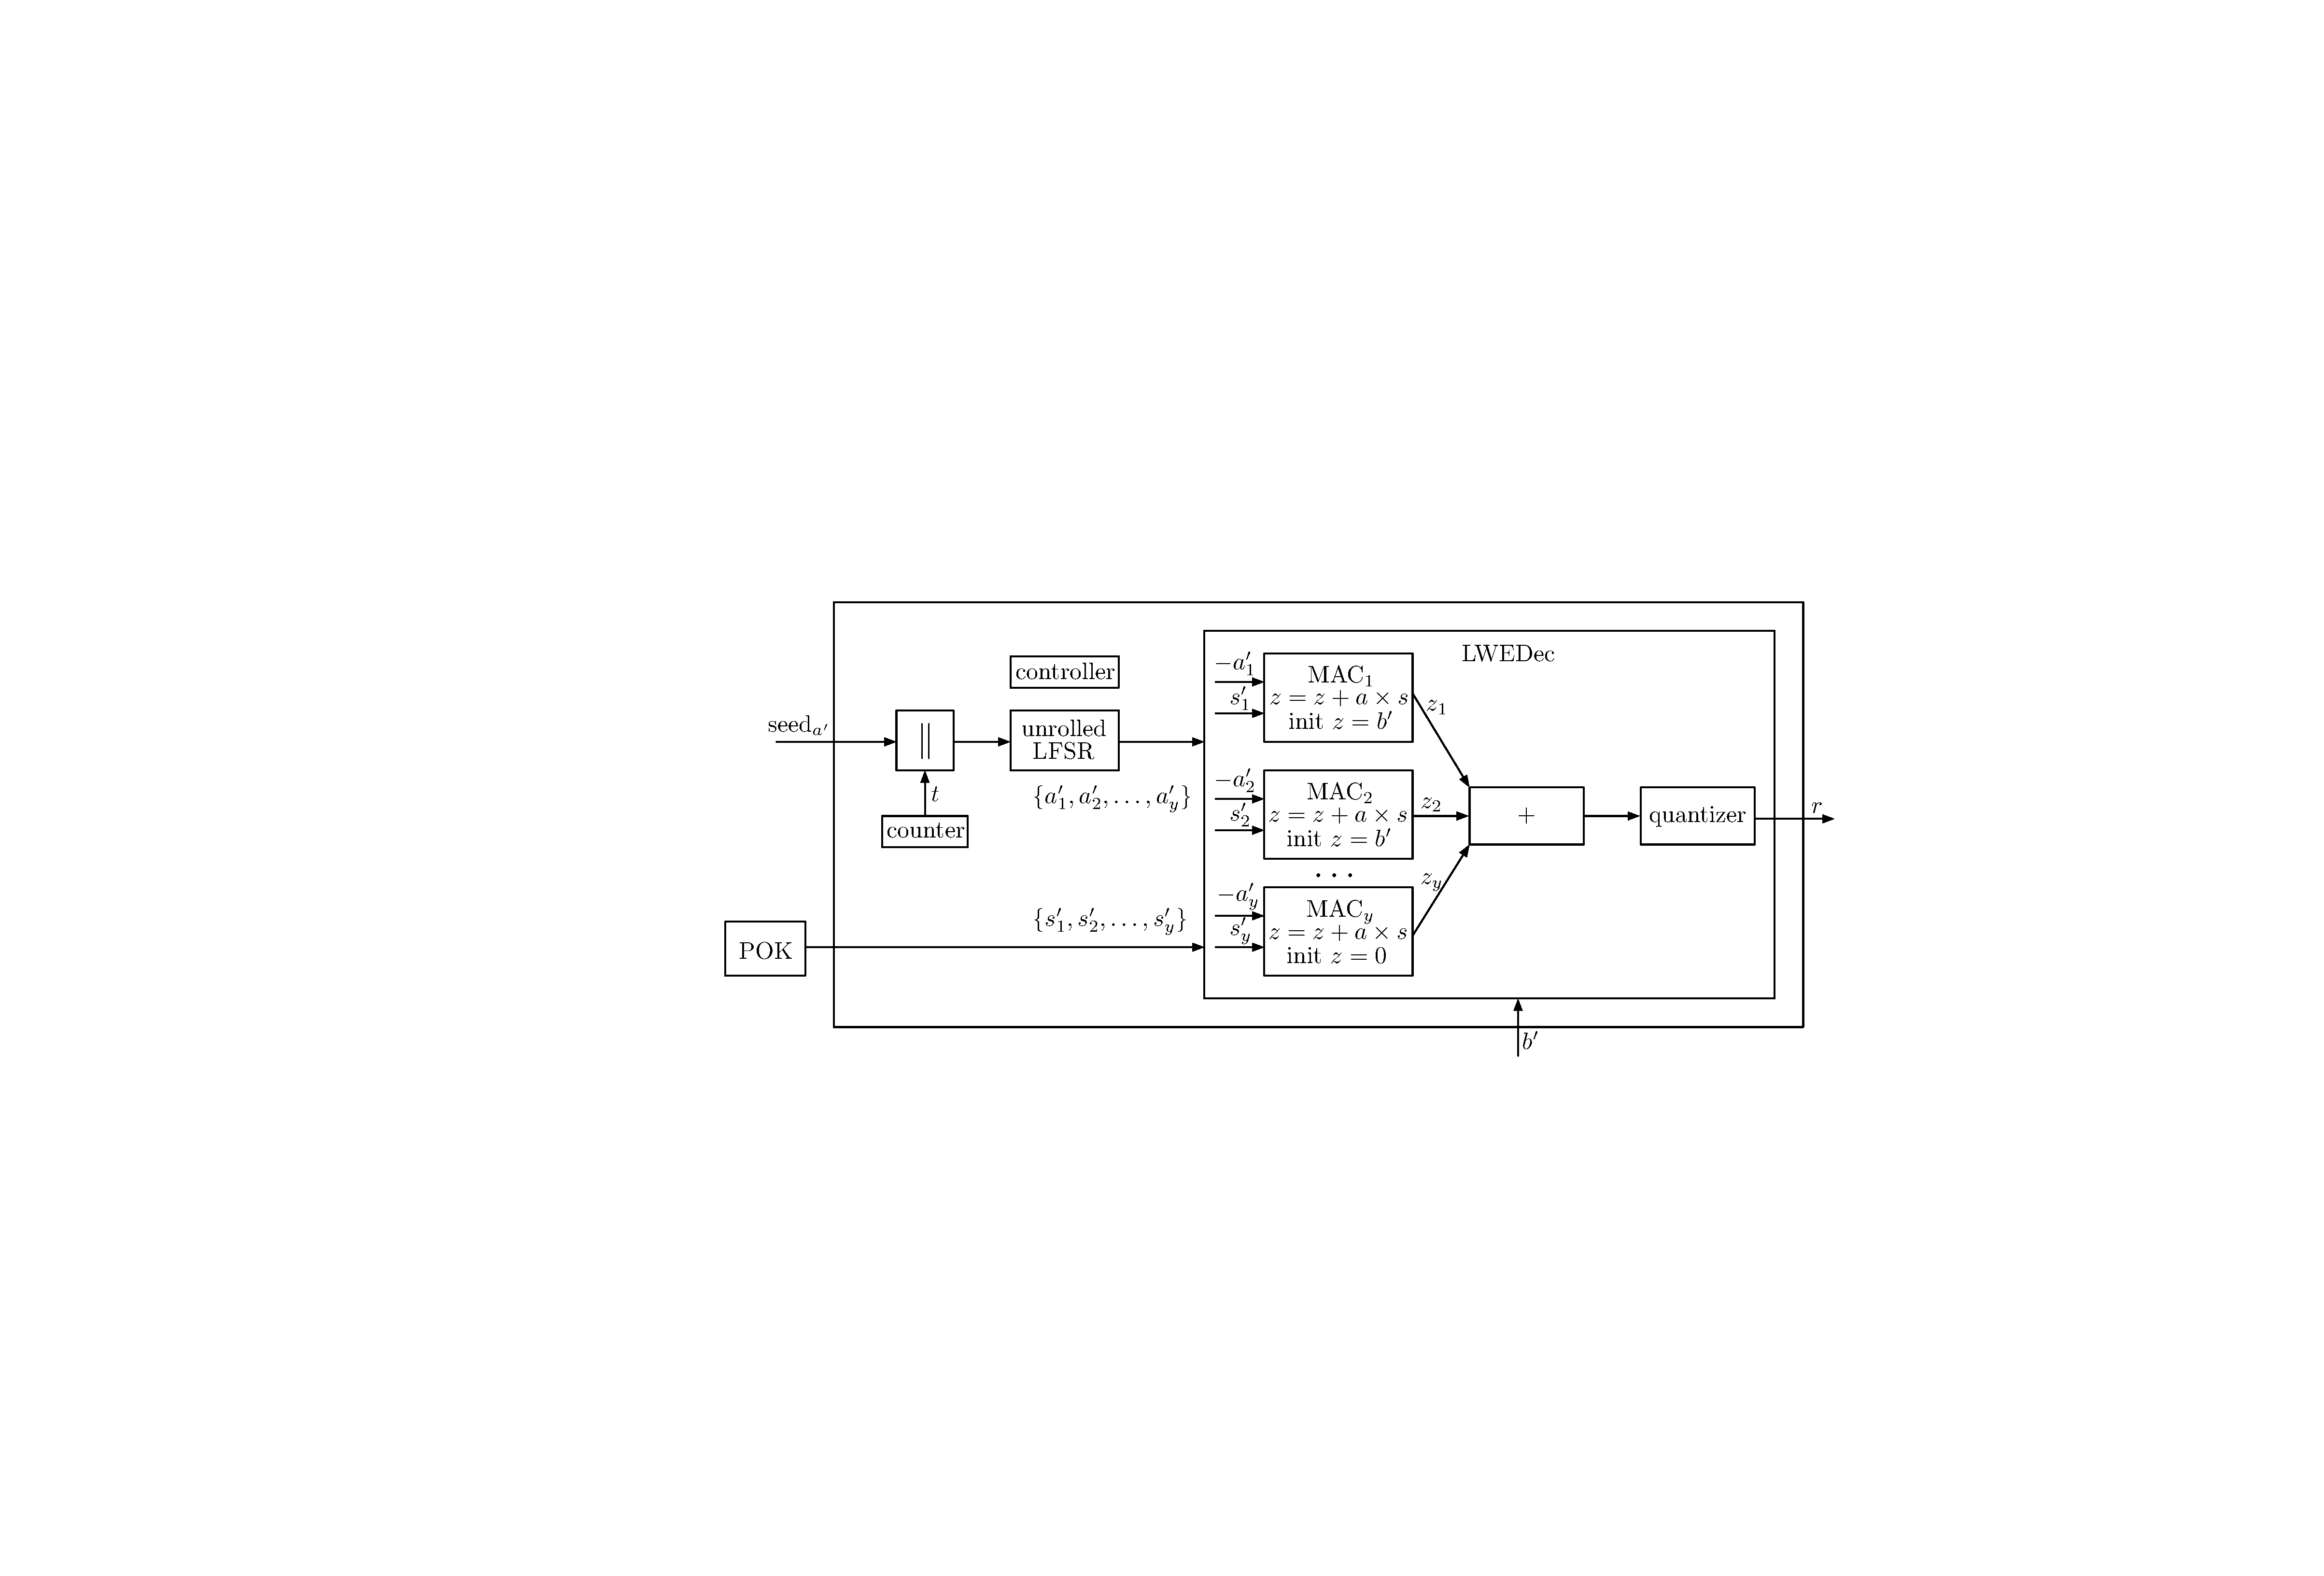
\includegraphics[width = 1.0\linewidth]{./figs/lpuf_p2_large}
\caption{Reducing latency via parallel MAC units.}
\label{fig:lpuf_p2}
\end{figure}

\begin{figure}[t!]
\centering
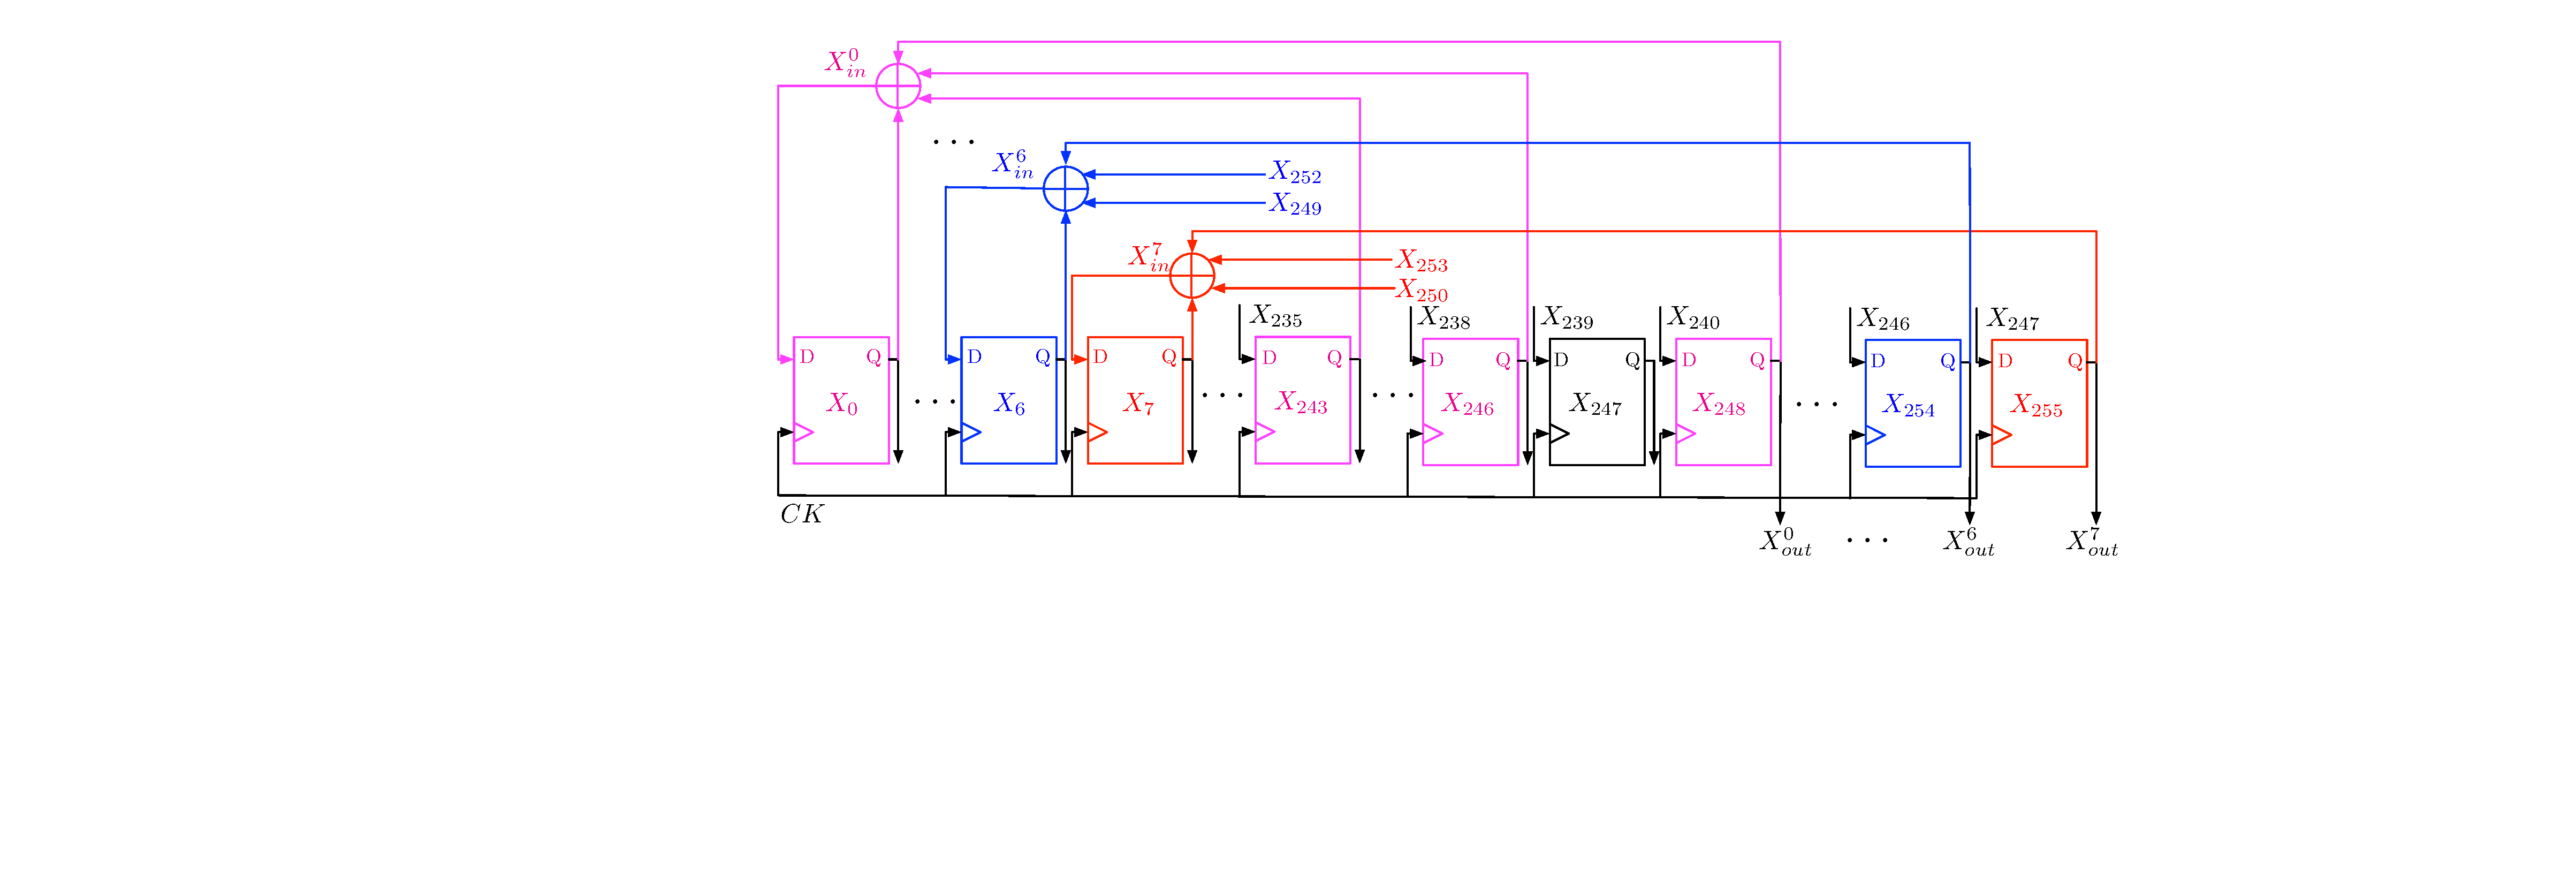
\includegraphics[width = 1.0\linewidth]{./figs/lfsr_unroll_limit_compressed}
\caption{The LFSR generator polynomial limits the maximum unrolling factor. It cannot produce feedback bits for more than $8$ consecutive cycles due to the constraint of $X_{7}$.}
\label{fig:lfsr_unrol_limit}
\end{figure}

An unrolled LFSR is functionally equivalent to the bit-serial LFSR, capable of producing multiple bits per cycle %\cite{cycle_efficient_lfsr, unrolled_lfsr_ref_2, unrolled_lfsr_ref_3}. 
\cite{cycle_efficient_lfsr, unrolled_lfsr_ref_2}. We adopt the basic loop unrolling strategy which completes the compute of multiple cycles within one cycle \cite{cycle_efficient_lfsr}.%The unrolling strategy is specific to the bit-serial implementation.} 

On each cycle, a bit-serial LFSR typically shifts the register bits by one position and shifts in one feedback bit, which is the XOR of higher register bits. A single output bit is produced. The basic idea of unrolling a LFSR is to parallelize the compute of multiple cycles to produce multiple output bits in one cycle. On each cycle, an unrolled LFSR completes the following tasks: computing the feedback bits of multiple consecutive cycles, shifting the register bits by multiple positions, loading the feedback bits to the multiple lowest registers, and assigning multiple output bits. 

We demonstrate how to unroll the 256-bit LFSR by a factor of 8. Fig. \ref{fig:lfsr_baseline} shows the LFSR implementation. The feedback bit is defined as $X_{in}$ and the output bit is defined as $X_{out}$. %($X_{255}$ to $X_{0}$ defines register bits)}
%\begin{equation*}
%    X_{in} = X_{255} \oplus X_{253} \oplus X_{250} \oplus X_{245} \\
%\end{equation*}
%\begin{equation*}
%    X_{out} = X_{255}
%\end{equation*}
We first compute feedback bits for 8 consecutive cycles:
\begin{align*}
    X_{in} ^ 7 &=  X_{255} \oplus X_{253} \oplus X_{250} \oplus X_{245} \\
    X_{in} ^ 6 &=  X_{254} \oplus X_{252} \oplus X_{249} \oplus X_{244} \\
    &\cdots \\
    X_{in} ^ 0 &= X_{248} \oplus X_{246} \oplus X_{243} \oplus X_{238}
\end{align*}

Then we modify the stride of the shift to update the register state after multiple single-position shifts. Besides the lowest 8 register bits, each register bit is updated with the bit value, located 8 bits away from the current bit:

\begin{equation*}
    X_{i} = X_{i-8}
\end{equation*}

The lowest 8 register bits latch values of the 8 feedback bits $X_{in} ^ 7$ to $X_{in} ^ 0$. Finally, we assign multiple register bits to output bits:
\begin{align*}
    X_{out} ^ 7 &=  X_{255} \\
    X_{out} ^ 6 &=  X_{254}  \\
    &\cdots \\
    X_{out} ^ 0 &= X_{248} 
\end{align*}

Fig. \ref{fig:lfsr_unrolled} shows the architecture of the unrolled LFSR. It improves the throughput of the baseline bit-serial LFSR by 8X, at the cost of more XOR gates for computation.

We implemented parallel MAC units in the LWE decryption function with an unrolled LFSR generating multiple bytes of ciphertext, Fig. \ref{fig:lpuf_p2}. We initialized the accumulation register of one of the MAC unit with ciphertext $b$, and the accumulation registers of the rest of MAC units to 0. On each cycle, each MAC unit accumulates the product of a byte of POK with the opposite of one byte of ciphertext $\mathbf{a}$ (Recall that the LWE decryption computes $b-\innerprod{\mathbf{a},\mathbf{s}}$). Finally the partial sums from each MAC unit are accumulated together to produce a dot-product result. The result is quantized and a response bit is produced. The increased number of MAC units reduces the number of MAC operations assigned to each unit, thus reducing the dot-product latency. On a design with $P_2$ parallel MAC units, the strategy reduces the dot-product latency for a response bit by a factor of $P_2$. The cost is the increase in hardware resource utilization due to an unrolled LFSR and the parallel MAC units.

The LFSR-LWEDec datapath parallelization and MAC unit parallelization can be combined. Specifically, each parallel LFSR-LWEDec datapath can adopt an unrolled LFSR and a LWE decryption function with multiple MAC units. In practice, a user selects $P_1$ and $P_2$ values based on the latency requirement, resource budget, and the baseline LFSR implementation. MAC unit parallelization is more resource-efficient since the strategy only needs additional hardware for unrolled LFSR and MAC units. In contrast, the LFSR-LWEDec data-path parallelization requires duplication of the entire datapath. 

However, the MAC unit parallelization cannot achieve arbitrary parallelism since the LFSR cannot be unrolled with an arbitrary factor. The LFSR generator polynomial limits the maximum unrolling factor, Fig. \ref{fig:lfsr_unrol_limit}. If the 256-bit LFSR takes the XOR result of $X_{255}$, $X_{253}$, $X_{250}$ and $X_{7}$ as the feedback bit, the LFSR cannot be unrolled by over 8 times with the demonstrated technique, since the LSB $X_{0}$ is only $7$ bits away from $X_{7}$. This indicates the unrolled LFSR cannot produce more than $8$ consecutive feedback bits utilizing consecutive register bits lower than $X_{7}$. The lowest LFSR bit involved in the feedback bit calculation determines the maximum unrolling times. LFSR-LWEDec data-path parallelization is a generic strategy. Its maximum parallelism is not constrained by any specific LFSR implementation. Therefore, in practice, the optimal strategy is to first seek parallelization via LFSR unrolling, and then parallelize the LFSR-LWEDec data-path to achieve further latency optimization once the unrolling of LFSR reaches the limit. We validate the strategy with a detailed design space exploration in Section \ref{sec:result}.

\begin{figure}[t!]
\centering
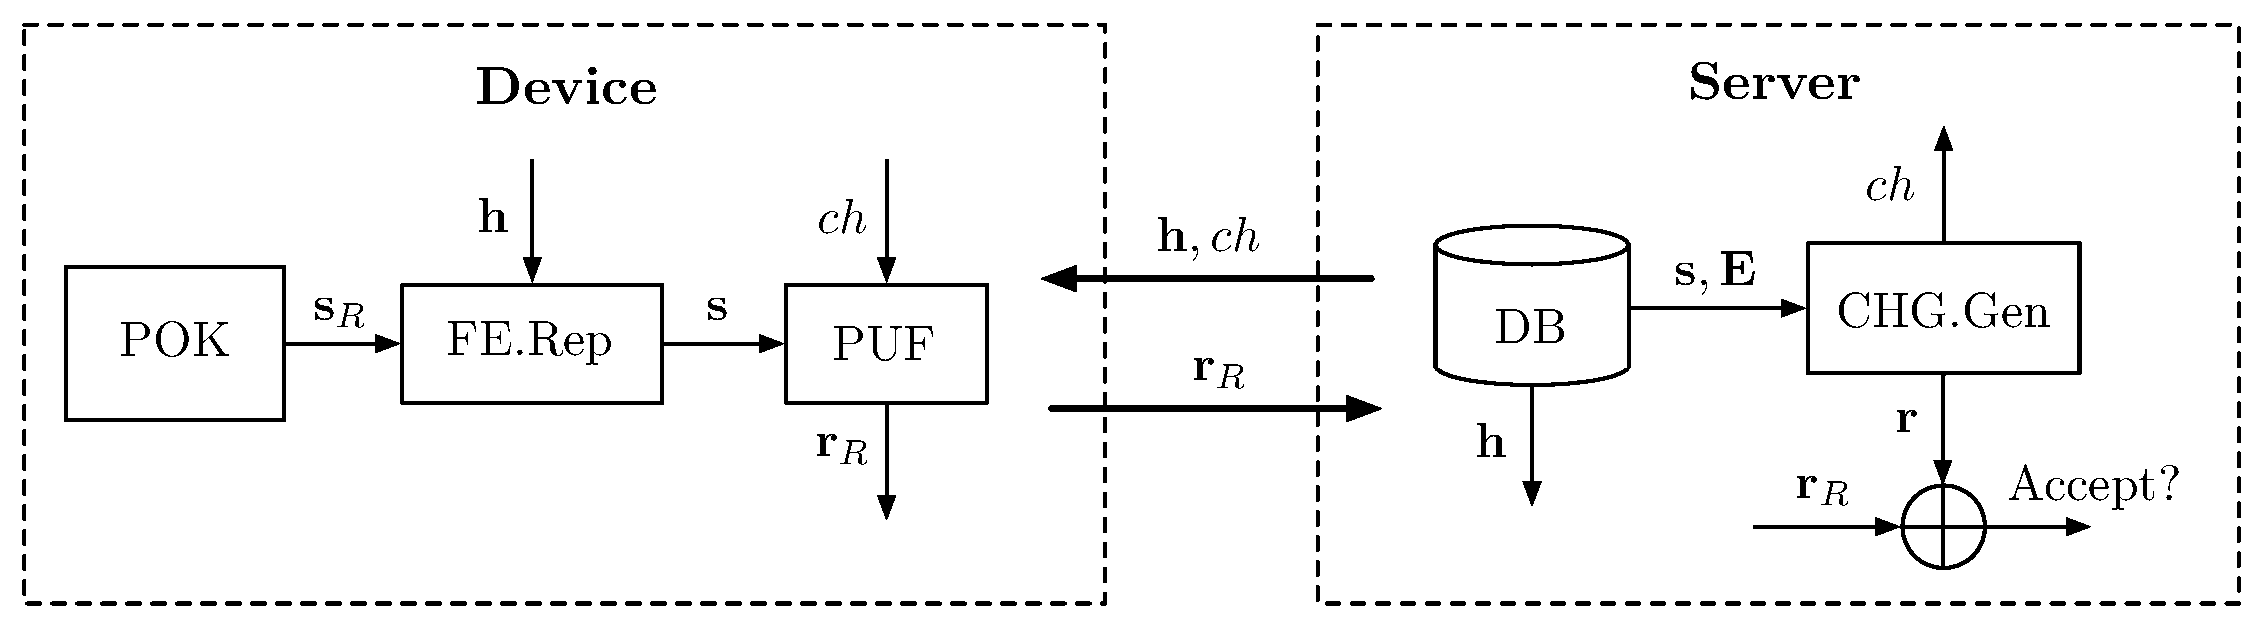
\includegraphics[width = 1.0\linewidth]{./figs/authen_system}
\caption{Building blocks of the authentication scheme with the lattice PUF.}
\label{fig:authen_system}
\end{figure}

\begin{figure}[t!]
\centering
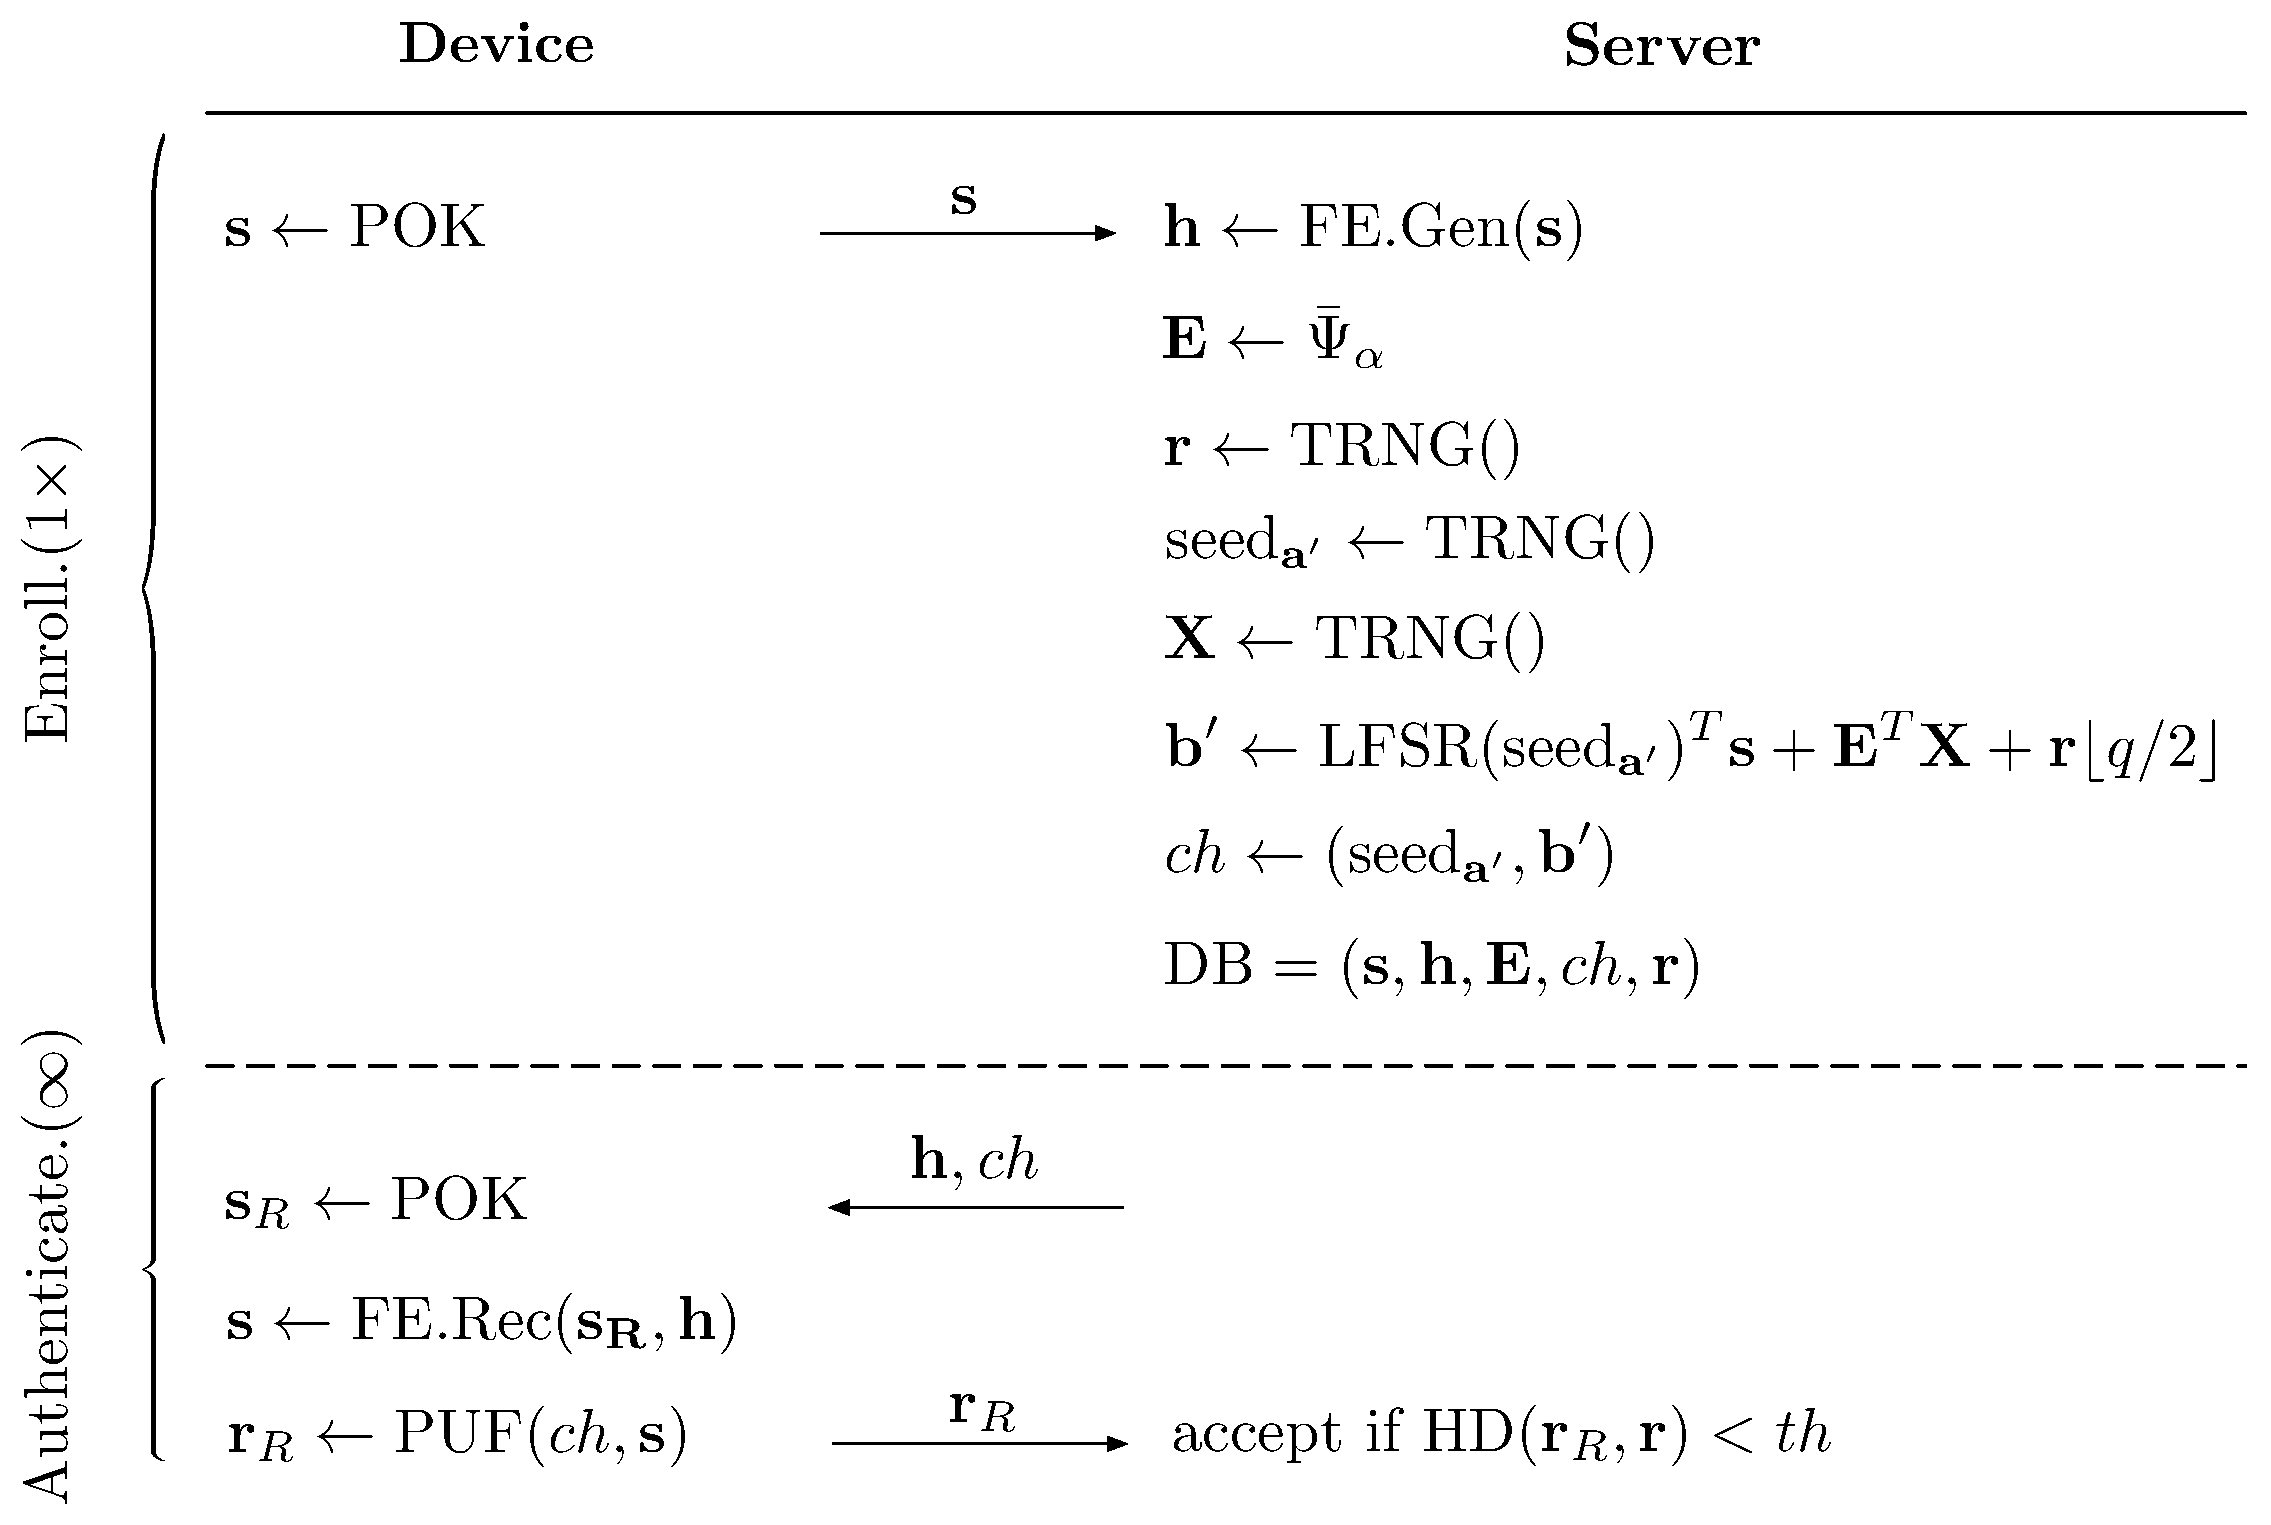
\includegraphics[width = 0.9\linewidth]{./figs/protocol}
\caption{End-to-end authentication method with the lattice PUF.}
\label{fig:protocol}
\end{figure}

\subsection{Application Scenario and Reverse Fuzzy Extractor}

To reconstruct stable POK bits, we adopt the fuzzy extractor (FE) \cite{bosch2008efficient} method to achieve a low failure rate. To reduce device-side complexity of design, we use a reverse fuzzy extractor (RFE) that moves the complex error correction process from the device to the server \cite{van2012reverse}. As an example application, we study using the lattice PUF in a string-matching authentication scheme \cite{suh2007physical}.

Figure \ref{fig:authen_system} shows the building blocks of an authentication scheme based on the lattice PUF. The device contains a POK generator, an RFE generation block (\texttt{RFE.Gen}), and a lattice PUF. The server has a database (\texttt{DB}) to store the POK, an RFE reconstruction block (\texttt{RFE.Rec}), and a server-side lattice PUF.

Our threat model assumes that the device operates in the field and is the target of ML attacks. We consider the server to be in a physically secure location, with the \texttt{DB} storing the POK bits and the sever-side lattice PUF being secret. %The adversary can eavesdrop on $ch$, $\mathbf{h}$, $r_R$. The RFE construction guarantees that there is sufficient left-over entropy on the secret key, and so disclosing helper data $\mathbf{h}$ is secure against state-of-the-art attacks \cite{delvaux2016efficient}.

Figure \ref{fig:protocol} shows the operations of an end-to-end authentication method using the lattice PUF. During the enrollment phase, the server reads out the POK $\mathbf{s}$ from the SRAM cells through a one-time interface, and stores it in the server \texttt{DB}. During each authentication, the error correction uses the code-offset construction with a concatenated code. Here the secret $\mathbf{t}$ is a nonce, which is encoded into a codeword $\mathbf{k}$ and then XORed with the SRAM bits $\mathbf{s}_R$ to produce the helper data $\mathbf{h}$. The server reverses these steps using the enrolled POK $\mathbf{s}$. If the HD between $\mathbf{s}$ and $\mathbf{s}_R$ is within the error-decoding capability of the ECC decoder, the server reconstructs the correct secret key $\mathbf{t}$. Finally, the server sends the challenge $ch=(\text{seed}_{\mathbf{a}^\prime}, \mathbf{b}')$ to the device. The device generates the PUF response $\mathbf{r}_R$ and sends it to the server. The server compares $\mathbf{r}_R$ with the response $\mathbf{r}$ generated from the server-side lattice PUF. The device will be accepted if $\text{HD}(\mathbf{r}_R, \mathbf{r})$ is less than a threshold $th$.

%\textcolor{red}{A class of attacks which manipulates public helper data to exploit PUF generated keys can compromise PUF security \cite{helper_data_manipulation}. Such attacks apply to pairing-based PUFs (for instance, RO PUFs), and require public access to helper data. However, such attacks may not be applicable to our construction, since our POK is based on the SRAM PUF, which follows a completely different mechanism. In addition, the possibility of the attacks can be reduced by limiting public access to helper data. Therefore, the helper data manipulation attack is not a major focus for our design.}